% ============================================================
%  Shared preamble - matches the Mode-0 report house style
% ============================================================
\documentclass[11pt,a4paper]{article}

\usepackage[utf8]{inputenc}
\usepackage[expansion=false]{microtype}
\usepackage[a4paper,left=28mm,right=28mm,top=28mm,bottom=25mm]{geometry}

\usepackage{amsmath,amssymb}
\usepackage{booktabs}
\usepackage{array}
\usepackage{enumitem}
\usepackage{xcolor}
\usepackage{caption}
\usepackage{fancyhdr}
\usepackage{titlesec}
\usepackage{tikz}
\usetikzlibrary{positioning,arrows.meta,calc,fit,backgrounds,shapes.geometric}
\usepackage[most]{tcolorbox}
\usepackage[section]{placeins}
\usepackage[hidelinks]{hyperref}

% ---------- colours ----------
\definecolor{navy}{RGB}{26,60,102}
\definecolor{accent}{RGB}{40,92,148}
\definecolor{softblue}{RGB}{232,240,248}
\definecolor{rulegrey}{RGB}{120,130,140}
\definecolor{orangeacc}{RGB}{196,106,48}
\definecolor{boxblue}{RGB}{219,232,244}
\definecolor{tealbox}{RGB}{214,236,238}
\definecolor{peachbox}{RGB}{250,226,208}
\definecolor{greybox}{RGB}{238,240,242}

\hypersetup{
  colorlinks=true,
  linkcolor=accent,
  urlcolor=accent,
  citecolor=accent,
  pdftitle={Bluetooth Channel Sounding Mode-1 Round-Trip-Time Estimation},
  pdfsubject={Formal technical report},
}

% ---------- headings ----------
\titleformat{\section}{\normalfont\Large\bfseries\color{navy}}{\thesection}{0.8em}{}
\titleformat{\subsection}{\normalfont\large\bfseries\color{navy}}{\thesubsection}{0.7em}{}
\titleformat{\subsubsection}{\normalfont\normalsize\bfseries\color{navy}}{\thesubsubsection}{0.6em}{}
\titlespacing*{\section}{0pt}{1.9\baselineskip}{0.8\baselineskip}
\titlespacing*{\subsection}{0pt}{1.2\baselineskip}{0.5\baselineskip}

% ---------- captions ----------
\captionsetup{font=small,labelfont={bf,color=accent},labelsep=colon,width=0.92\textwidth}
\captionsetup[table]{position=above,skip=4pt}
\captionsetup[figure]{position=below,skip=8pt}

% ---------- headers ----------
\pagestyle{fancy}
\fancyhf{}
\renewcommand{\headrulewidth}{0.6pt}
\fancyhead[L]{\small Bluetooth CS Mode-1 RTT Estimation}
\fancyhead[R]{\small Formal technical report - Revision 1.0}
\fancyfoot[C]{\small\thepage}

% ---------- callout box ----------
\newtcolorbox{callout}[1][]{
  colback=softblue, colframe=accent, boxrule=0.5pt,
  left=6pt,right=6pt,top=5pt,bottom=5pt, arc=1pt,
  fontupper=\small, #1}

% ---------- table helpers ----------
\newcolumntype{L}[1]{>{\raggedright\arraybackslash}p{#1}}
\renewcommand{\arraystretch}{1.18}

% ---------- macros ----------
\newcommand{\us}{\,\ensuremath{\upmu}s}
\newcommand{\ToD}{\mathrm{ToD}}
\newcommand{\ToA}{\mathrm{ToA}}
\newcommand{\ToF}{\mathrm{ToF}}
\newcommand{\RTT}{\mathrm{RTT}}
\newcommand{\FFO}{\mathrm{FFO}}
\newcommand{\NADM}{\mathrm{NADM}}
\newcommand{\Tsy}{T_{SY}}
\newcommand{\Trd}{T_{RD}}
\newcommand{\Tip}{T_{IP1}}
\newcommand{\code}[1]{\texttt{\small #1}}
\providecommand{\upmu}{\mu}

% TikZ block styles reused across figures
\tikzset{
  blk/.style   ={draw=navy!70, fill=softblue, rounded corners=1pt, align=center,
                 font=\scriptsize, inner sep=3.5pt, minimum height=8mm},
  pblk/.style  ={draw=navy!70, fill=white, rounded corners=1pt, align=center,
                 font=\scriptsize, inner sep=3.5pt, minimum height=8mm},
  ar/.style    ={-{Latex[length=2mm]}, draw=navy!80, thick},
  dar/.style   ={-{Latex[length=2mm]}, draw=orangeacc, dashed, thin},
  slot/.style  ={draw=navy!55, font=\scriptsize, align=center, minimum height=7mm},
}
% ============================================================
%  Front matter and Sections 1-7
% ============================================================
\begin{document}

% ---------------- Title page ----------------
\thispagestyle{empty}
\vspace*{18mm}
{\color{accent}\small\bfseries FORMAL TECHNICAL REPORT \hfill REVISION 1.0}

\vspace{26mm}
{\raggedright\color{navy}\Huge\bfseries Bluetooth Channel Sounding\par}
\vspace{5mm}
{\raggedright\color{navy}\huge\bfseries Mode-1 Round-Trip-Time Estimation\par}

\vspace{7mm}
\noindent{\raggedright\color{rulegrey}\large Timestamp formation, time-of-arrival estimators,
clock-scale correction, and the RTT-to-distance chain\par}

\vspace{12mm}
\noindent\rule{\textwidth}{1pt}

\vspace{4mm}
\noindent
This report traces the complete measurement chain of a Bluetooth Channel Sounding Mode-1
step: the reciprocal \code{CS\_SYNC} exchange, the four local timestamps
$\ToD_I$, $\ToA_R$, $\ToD_R$, $\ToA_I$, their combination into a round-trip time, and the
conversion of that time into a distance. It derives the time-of-arrival estimation problem
from the GFSK signal model and develops the family of estimators that can serve it:
matched-filter correlation, sub-sample interpolation, early--late tracking, maximum-likelihood
and Cram\'er--Rao analysis, frequency-domain group-delay regression, first-path detection under
multipath, and super-resolution methods. It shows why transmitter and receiver group delays
\emph{add} rather than cancel in RTT, why Mode-0 frequency calibration is a prerequisite for
Mode-1 accuracy, and how the sounding sequence and the Normalized Attack Detector Metric relate
to timing integrity.

\vfill
\noindent
\begin{tabular}{@{}L{40mm}L{95mm}@{}}
Primary references & Core 6.3, Vol.\ 6, Part H, Sec.\ 4.3.2 and 4.4; Vol.\ 1, Part A, Sec.\ 9.1 \\
Air-interface timing & Core 6.3, Vol.\ 6, Part H, Secs.\ 4.3 and 4.5 \\
Companion report & \emph{Bluetooth CS Mode-0 Frequency Estimation}, Revision 3.0 \\
Document type & Scientific and implementation-oriented technical report \\
Revision date & 4 September 2026 \\
\end{tabular}

\newpage
\pagenumbering{roman}

% ---------------- Abstract ----------------
\section*{Abstract}
\addcontentsline{toc}{section}{Abstract}

Mode-1 is the round-trip-time step of Bluetooth Low Energy Channel Sounding. The initiator
transmits a \code{CS\_SYNC} packet, the reflector receives it and after the configured interlude
period $\Tip$ transmits its own \code{CS\_SYNC} packet on the same channel. Each device
timestamps its own departure and arrival events against its own clock. The four timestamps are
combined into a round-trip time whose ideal value is twice the one-way time of flight, and the
distance follows as $d = c\,\RTT/2$.

The specification defines the exchange, the permitted timing parameters, the \code{CS\_SYNC}
packet variants, and the reported timing observables. It does not mandate how a receiver
estimates the time of arrival of a GFSK packet. This report therefore separates normative
behaviour from receiver design. It derives the RTT equation from antenna-referenced event times,
shows that the four hardware group delays accumulate into a single additive loop delay that must
be calibrated rather than assumed to cancel, and shows that the reflector's turnaround interval
is measured on a different frequency scale and must be rescaled by the Mode-0 fractional
frequency offset before subtraction.

A dedicated section develops the time-of-arrival estimator family with explicit equations,
ambiguity and bias properties, and the Cram\'er--Rao bound that ties timing variance to
root-mean-square bandwidth and accumulated signal-to-noise ratio. A worked example at
2\,440\,MHz on the LE 2M PHY quantifies the achievable single-step and aggregated ranging
uncertainty, the cost of an uncorrected clock scale error, and the reporting quantum. The report
closes with an error budget, a layered verification plan, and the boundary between specified
behaviour and implementation choice.

\begin{callout}
\textbf{Status and interpretation.} Normative claims are tied to the cited Bluetooth Core
Specification sections. Signal-processing estimators, quality metrics, calibration databases and
aggregation rules are representative implementation methods. Timing parameter value lists and
report field encodings should be read from the adopted specification revision in force; where
this report states them, they are given to make the equations concrete. The Bluetooth
specification and adopted test specifications remain authoritative for conformance.
\end{callout}

\newpage
\tableofcontents
\newpage
\pagenumbering{arabic}
\setcounter{page}{1}

% ============================================================
\section{Scope and measurement objective}
% ============================================================

Bluetooth Channel Sounding uses several step modes. Mode-0 establishes the relative frequency
and timing scale between the two devices. Mode-1 uses that scale to measure a round-trip time.
Mode-2 measures phase on tone exchanges. Mode-3 combines a Mode-1-like packet exchange with
Mode-2-like tone exchanges in a single step.

The Mode-1 measurement objective is not a distance and not a raw counter value. It is the pair of
\emph{locally measured intervals}
\[
A_I \;=\; \ToA_I - \ToD_I \quad\text{(initiator)}, \qquad
B_R \;=\; \ToD_R - \ToA_R \quad\text{(reflector)},
\]
each expressed in its own device's calibrated time base, together with enough metadata to
combine them. The engineering chain is

\begin{enumerate}[leftmargin=1.6em,itemsep=1pt]
  \item identify the valid \code{CS\_SYNC} reception and estimate its time of arrival;
  \item convert receiver-chain and transmitter-chain marks to antenna-referenced event times;
  \item express both device intervals on a common frequency scale using the Mode-0 result;
  \item subtract the reflector interval from the initiator interval to form the round-trip time;
  \item remove the calibrated loop delay and convert to a one-way time of flight; and
  \item aggregate valid steps, gate outliers, and hand the result to the ranging algorithm.
\end{enumerate}

\subsection{What Mode-1 measures and what it does not}

Mode-1 produces an \emph{unambiguous} but comparatively coarse distance estimate. Its resolution
is limited by the occupied bandwidth of a single \code{CS\_SYNC} packet, roughly 2\,MHz, whose
reciprocal is about 500\,ns of delay resolution, or some 75\,m of distance. What makes Mode-1
useful is not resolution but \emph{estimation accuracy}: with adequate signal-to-noise ratio the
peak of a known waveform can be located to a small fraction of its own width, so the achievable
timing standard deviation is orders of magnitude below $1/B$.

Phase-based ranging in Mode-2 and Mode-3 has the opposite character. It synthesises an aperture
across the whole hopped band and therefore has fine resolution, but the phase observable is
periodic and yields an ambiguous distance. The architectural relationship is complementary and is
made explicit in Section~\ref{sec:fusion}.

\begin{callout}
\textbf{Three properties that are frequently confused.} (1) Mode-1 timing \emph{resolution} is set
by packet bandwidth; Mode-1 timing \emph{precision} is set by bandwidth and accumulated SNR
jointly. (2) Transmit and receive group delays do not cancel in the round-trip construction; they
add. (3) The reflector's turnaround interval is measured with the reflector's clock and is not
directly subtractable from an interval measured with the initiator's clock.
\end{callout}

% ============================================================
\section{Normative framework and terminology}
% ============================================================

The physical-layer definitions must be read together with the architectural description. Core 6.3
Volume 1, Part A, Section 9.1 states that the first CS steps provide calibration information and
identifies Mode-0 as calibration of one device to the other in frequency and timing. Mode-1 is the
first step mode that produces a ranging observable.

\begin{table}[h]
\caption{Normative map for the Mode-1 round-trip-time measurement.}
\label{tab:normmap}
\centering\small
\begin{tabular}{@{}L{40mm}L{52mm}L{52mm}@{}}
\toprule
Source & What it defines & Question answered \\
\midrule
Core 6.3, Vol.\ 1, Part A, Sec.\ 9.1 & CS procedure architecture; role of RTT in the ranging chain & Why is Mode-1 performed after Mode-0? \\
Core 6.3, Vol.\ 6, Part H, Sec.\ 4.3.2 & Mode-1 step packet order and timing & What is transmitted, in which order, and when? \\
Core 6.3, Vol.\ 6, Part H, Sec.\ 4.3 & $\Tsy$, $\Trd$, $\Tip$, $T_{FCS}$ and the permitted value sets & Which step timings may be configured? \\
Core 6.3, Vol.\ 6, Part H, Sec.\ 4.4 & \code{CS\_SYNC} packet construction: access address, trailer, sounding sequence, random sequence & What waveform is the receiver matched to? \\
Core 6.3, Vol.\ 6, Part A, Sec.\ 3.5 & Frequency measurement and generation in CS; expected frequencies for non-Mode-0 transmissions & On what carrier is the Mode-1 packet expected? \\
Core 6.3, Vol.\ 4, Part E, LE CS Subevent Result event & Per-step reported timing and quality fields & How is the measurement exposed to the host? \\
RFPHY.TS, CS step Mode-1 clauses & Instrument-level verification of RTT timing accuracy & How is the transmitted/received timing tested? \\
\bottomrule
\end{tabular}
\end{table}

\begin{table}[h]
\caption{Principal symbols.}
\label{tab:symbols}
\centering\small
\begin{tabular}{@{}L{28mm}L{78mm}L{22mm}@{}}
\toprule
Symbol & Meaning & Units \\
\midrule
$\ToD_I,\ \ToA_I$ & Initiator local departure and arrival timestamps & s \\
$\ToA_R,\ \ToD_R$ & Reflector local arrival and departure timestamps & s \\
$A_I$ & Initiator-measured round interval $\ToA_I-\ToD_I$ & s \\
$B_R$ & Reflector-measured turnaround interval $\ToD_R-\ToA_R$ & s \\
$\RTT$ & Round-trip time after correction & s \\
$\ToF$ & One-way time of flight & s \\
$D_{TX,X},\ D_{RX,X}$ & Transmit / receive chain group delay of device $X$ & s \\
$D_{loop}$ & Total calibrated loop delay & s \\
$\FFO^{*}_{RX}$ & Subevent fractional frequency offset from Mode-0 & ppm \\
$\Tsy$ & \code{CS\_SYNC} packet duration & s \\
$\Trd$ & Transmitter ramp-down period & s \\
$\Tip$ & Interlude period between initiator and reflector transmissions & s \\
$s(t)$ & Known transmitted complex envelope of \code{CS\_SYNC} & --- \\
$z[n]$ & Received complex baseband sample & ADC units \\
$R(\tau)$ & Cross-correlation of $z$ with the reference $s$ & --- \\
$\tau_\ell,\ a_\ell$ & Delay and complex gain of multipath component $\ell$ & s, --- \\
$\beta_{rms}$ & Root-mean-square bandwidth of $s(t)$ & Hz \\
$\NADM$ & Normalized Attack Detector Metric & index \\
\bottomrule
\end{tabular}
\end{table}

% ============================================================
\section{Position of Mode-1 in the CS subevent}
% ============================================================

Figure~\ref{fig:stack} places Mode-1 in the causal chain. Mode-0 runs first and produces the
subevent frequency reference $\FFO^{*}_{RX}$. That reference is used for two distinct purposes in
Mode-1: it places the expected carrier so the packet is received with small residual frequency
offset, and it converts the reflector's measured turnaround interval onto the initiator's time
scale.

\begin{figure}[h]
\centering
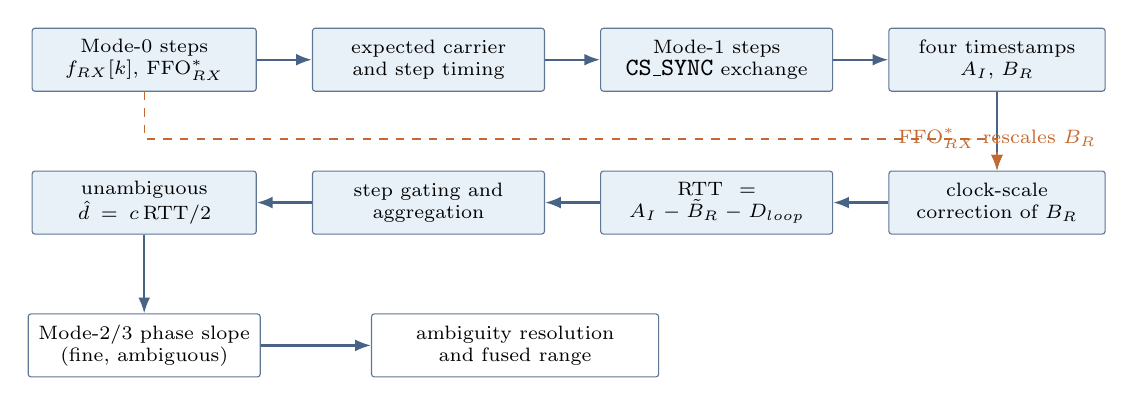
\begin{tikzpicture}[node distance=6mm and 7mm]
\node[blk,text width=26mm] (m0) {Mode-0 steps\\ $f_{RX}[k]$, $\FFO^{*}_{RX}$};
\node[blk,right=of m0,text width=27mm] (carr) {expected carrier\\ and step timing};
\node[blk,right=of carr,text width=27mm] (m1) {Mode-1 steps\\ \code{CS\_SYNC} exchange};
\node[blk,right=of m1,text width=25mm] (ts) {four timestamps\\ $A_I$, $B_R$};

\node[blk,below=10mm of ts,text width=25mm] (scale) {clock-scale\\ correction of $B_R$};
\node[blk,left=of scale,text width=27mm] (rtt) {$\RTT = A_I - \tilde B_R - D_{loop}$};
\node[blk,left=of rtt,text width=27mm] (agg) {step gating and\\ aggregation};
\node[blk,left=of agg,text width=26mm] (dist) {unambiguous\\ $\hat d = c\,\RTT/2$};

\node[pblk,below=10mm of dist,text width=27mm] (pbr) {Mode-2/3 phase slope\\ (fine, ambiguous)};
\node[pblk,right=14mm of pbr,text width=34mm] (fuse) {ambiguity resolution\\ and fused range};

\draw[ar] (m0)--(carr); \draw[ar] (carr)--(m1); \draw[ar] (m1)--(ts);
\draw[ar] (ts)--(scale); \draw[ar] (scale)--(rtt); \draw[ar] (rtt)--(agg); \draw[ar] (agg)--(dist);
\draw[ar] (dist)--(pbr.north-|dist);
\draw[ar] (pbr)--(fuse);
\draw[dar] (m0.south) |- ($(scale.north)+(0,4mm)$) -- (scale.north)
   node[midway,above,font=\scriptsize,color=orangeacc,pos=0.62] {$\FFO^{*}_{RX}$ rescales $B_R$};
\end{tikzpicture}
\caption{Position of Mode-1. Mode-0 supplies both the expected carrier and the frequency scale
used to rescale the reflector interval. Mode-1 produces an unambiguous range which subsequently
resolves the ambiguity of the phase-based estimate.}
\label{fig:stack}
\end{figure}

\subsection{Why Mode-1 cannot precede Mode-0}

Two independent effects make the ordering mandatory rather than conventional.

\emph{Carrier placement.} A receiver that has not measured the peer's frequency error must open a
wide acquisition range. Residual carrier offset degrades coherent correlation over the packet: a
residual $\delta f$ rotates the correlator integrand by $2\pi\,\delta f\,T_{obs}$ across an
observation of length $T_{obs}$, and once that rotation approaches one cycle the coherent gain
collapses. For a 96-bit sounding sequence at 2\,Mb/s, $T_{obs}=48\us$, so a residual of
$10\,\text{kHz}$ already produces about half a cycle of rotation.

\emph{Interval scale.} The reflector reports an interval measured with its own oscillator. If that
oscillator differs in rate by $\epsilon$, the reported interval is wrong by $\epsilon\,B_R$. With
$B_R \approx 224\us$, the value reached in Section~\ref{sec:example}, and $\epsilon = 12$\,ppm, the
error is $2.69$\,ns, which is $40$\,cm of range. Section~\ref{sec:clock} develops this.

% ============================================================
\section{Mode-1 timing and the valid measurement interval}
% ============================================================

\subsection{One complete Mode-1 step}

Figure~\ref{fig:m1timing} shows the air-interface order of a Mode-1 step. Widths are labelled
rather than drawn to scale, because $\Tsy$ depends on the selected CS synchronization PHY and RTT
type, and $\Tip$ is configured.

\begin{figure}[h]
\centering
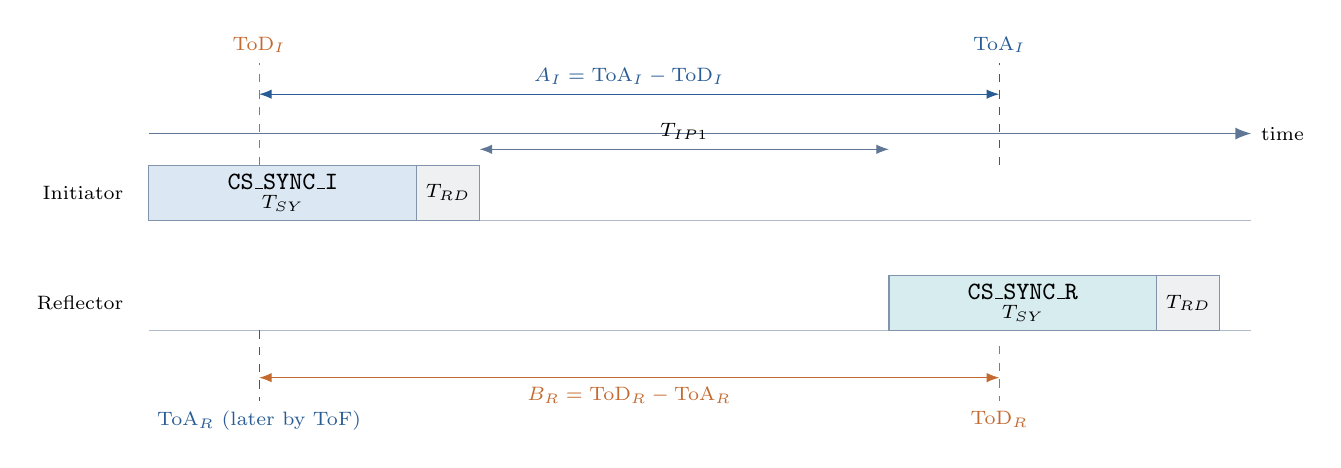
\begin{tikzpicture}[x=1mm,y=1mm]
\def\yI{14} \def\yR{0}
% axes
\draw[-{Latex[length=2mm]},draw=navy!70] (0,\yI+11) -- (140,\yI+11) node[right,font=\scriptsize] {time};
\node[font=\scriptsize,anchor=east] at (-2,\yI+3.5) {Initiator};
\node[font=\scriptsize,anchor=east] at (-2,\yR+3.5) {Reflector};
\draw[draw=navy!35] (0,\yI) -- (140,\yI);
\draw[draw=navy!35] (0,\yR) -- (140,\yR);

% initiator TX
\draw[slot,fill=boxblue] (0,\yI) rectangle (34,\yI+7)
   node[midway,align=center] {\code{CS\_SYNC\_I}\\[-1pt] $\Tsy$};
\draw[slot,fill=greybox] (34,\yI) rectangle (42,\yI+7) node[midway] {$\Trd$};

% reflector TX
\draw[slot,fill=tealbox] (94,\yR) rectangle (128,\yR+7)
   node[midway,align=center] {\code{CS\_SYNC\_R}\\[-1pt] $\Tsy$};
\draw[slot,fill=greybox] (128,\yR) rectangle (136,\yR+7) node[midway] {$\Trd$};

% interlude bracket
\draw[{Latex[length=1.6mm]}-{Latex[length=1.6mm]},draw=navy!70] (42,\yI+9) -- (94,\yI+9)
   node[midway,above,font=\scriptsize] {$\Tip$};

% timestamps
\draw[dashed,draw=orangeacc] (14,\yI+7) -- (14,\yI+20);
\node[font=\scriptsize,color=orangeacc,anchor=south] at (14,\yI+20) {$\ToD_I$};
\draw[dashed,draw=orangeacc] (108,\yR-2) -- (108,\yR-9);
\node[font=\scriptsize,color=orangeacc,anchor=north] at (108,\yR-9) {$\ToD_R$};
\draw[dashed,draw=accent] (14,\yR) -- (14,\yR-9);
\node[font=\scriptsize,color=accent,anchor=north] at (14,\yR-9) {$\ToA_R$ (later by $\ToF$)};
\draw[dashed,draw=accent] (108,\yI+7) -- (108,\yI+20);
\node[font=\scriptsize,color=accent,anchor=south] at (108,\yI+20) {$\ToA_I$};

% measured intervals
\draw[{Latex[length=1.6mm]}-{Latex[length=1.6mm]},draw=accent] (14,\yI+16) -- (108,\yI+16)
   node[midway,above,font=\scriptsize,color=accent] {$A_I=\ToA_I-\ToD_I$};
\draw[{Latex[length=1.6mm]}-{Latex[length=1.6mm]},draw=orangeacc] (14,\yR-6) -- (108,\yR-6)
   node[midway,below,font=\scriptsize,color=orangeacc] {$B_R=\ToD_R-\ToA_R$};
\end{tikzpicture}
\caption{Mode-1 step. The initiator transmits \code{CS\_SYNC}, ramps down, and after the
interlude period $\Tip$ the reflector transmits its own \code{CS\_SYNC} on the same channel.
Each device timestamps only its own two events, against its own clock.}
\label{fig:m1timing}
\end{figure}

The nominal step duration is
\begin{equation}
T_{step,1} \;=\; 2\Tsy + 2\Trd + \Tip ,
\label{eq:stepdur}
\end{equation}
with the frequency-change period $T_{FCS}$ inserted between scheduled steps when consecutive steps
use different channels. Note the structural difference from Mode-0: there is no separate guard
period $T_{GD}$ and no tone period $T_{FM}$, because Mode-1 carries no tone.

\subsection{Timing parameters}

\begin{table}[h]
\caption{Mode-1 step timing parameters. Permitted sets are configuration-dependent and are subject
to both devices' declared capabilities; read the value lists from the specification revision in
force.}
\label{tab:timing}
\centering\small
\begin{tabular}{@{}L{20mm}L{58mm}L{50mm}@{}}
\toprule
Parameter & Meaning & Representative permitted values \\
\midrule
$\Tsy$   & \code{CS\_SYNC} packet duration & PHY- and RTT-type-dependent; see Table~\ref{tab:tsy} \\
$\Trd$   & Transmitter ramp-down & $5\us$ \\
$\Tip$   & Interlude period, end of initiator ramp-down to start of reflector packet & $10,20,30,40,50,60,80,145\us$ \\
$T_{FCS}$& Frequency-change period between steps & $15,20,30,40,50,60,80,100,120,150\us$ \\
\bottomrule
\end{tabular}
\end{table}

$\Tsy$ follows from the packet construction of Section~\ref{sec:packet} and the symbol rate of the
selected CS synchronization PHY:
\begin{equation}
\Tsy \;=\; \frac{N_{pre} + N_{AA} + N_{tr} + N_{seq}}{R_b},
\label{eq:tsy}
\end{equation}
with $N_{AA}=32$ access-address bits, $N_{tr}=4$ trailer bits, $N_{pre}=8$ on the LE 1M PHY and
$16$ on the LE 2M PHYs, and $N_{seq}$ the length of the optional sounding or random sequence.

\begin{table}[h]
\caption{Packet duration $\Tsy$ from Eq.~\eqref{eq:tsy}. Values are derived from the packet
structure and symbol rate; the specification's timing table is authoritative.}
\label{tab:tsy}
\centering\small
\begin{tabular}{@{}L{30mm}rrrrr@{}}
\toprule
Sequence option & none & 32-bit & 64-bit & 96-bit & 128-bit \\
\midrule
Bits (LE 1M) & 44 & 76 & 108 & 140 & 172 \\
$\Tsy$ (LE 1M) & $44\us$ & $76\us$ & $108\us$ & $140\us$ & $172\us$ \\[2pt]
Bits (LE 2M) & 52 & 84 & 116 & 148 & 180 \\
$\Tsy$ (LE 2M) & $26\us$ & $42\us$ & $58\us$ & $74\us$ & $90\us$ \\
\bottomrule
\end{tabular}
\end{table}

\subsection{The reciprocal structure of the exchange}

The essential property of the Mode-1 step is that the same physical propagation delay appears
twice, once in each direction, while the reflector's turnaround interval appears with a sign that
lets it be removed. The four transmit and receive chain delays do \emph{not} enjoy that property;
Section~\ref{sec:groupdelay} shows that they accumulate instead. Specifically, the reflector's
turnaround time -- which is dominated by the configured
$\Tip$ and is not known to nanosecond accuracy a priori -- cancels because the reflector
\emph{measures} it and reports it, rather than the initiator assuming it.

\subsection{Repeated Mode-1 steps}

A CS subevent contains $M$ Mode-1 steps, generally on different channels. Each step yields an
independent $\RTT$ estimate. Because the timing observable is a delay and not a phase, per-step
values may be combined directly across channels, unlike the Mode-0 case where hertz values must
first be converted to a dimensionless offset. The caveat is that transmit and receive group delay
is channel-dependent, so a per-channel calibration table is required before aggregation
(Section~\ref{sec:groupdelay}).

% ============================================================
\section{The \code{CS\_SYNC} packet and RTT types}
\label{sec:packet}
% ============================================================

\subsection{Packet structure}

The \code{CS\_SYNC} packet is deliberately minimal. It carries no header, no length field, and no
CRC. Its purpose is to be a known waveform whose arrival time can be estimated.

\begin{figure}[h]
\centering
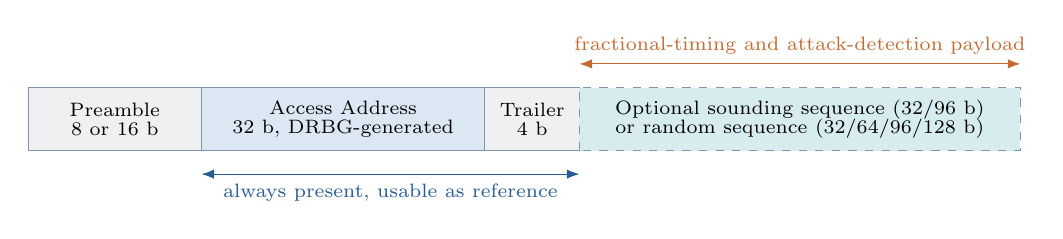
\begin{tikzpicture}[x=1mm,y=1mm]
\draw[slot,fill=greybox]  (0,0)  rectangle (22,8) node[midway,align=center] {Preamble\\[-1pt] 8 or 16 b};
\draw[slot,fill=boxblue]  (22,0) rectangle (58,8) node[midway,align=center] {Access Address\\[-1pt] 32 b, DRBG-generated};
\draw[slot,fill=greybox]  (58,0) rectangle (70,8) node[midway,align=center] {Trailer\\[-1pt] 4 b};
\draw[slot,fill=tealbox,dashed] (70,0) rectangle (126,8)
      node[midway,align=center] {Optional sounding sequence (32/96 b)\\[-1pt] or random sequence (32/64/96/128 b)};
\draw[{Latex[length=1.6mm]}-{Latex[length=1.6mm]},draw=accent] (22,-3) -- (70,-3)
   node[midway,below,font=\scriptsize,color=accent] {always present, usable as reference};
\draw[{Latex[length=1.6mm]}-{Latex[length=1.6mm]},draw=orangeacc] (70,11) -- (126,11)
   node[midway,above,font=\scriptsize,color=orangeacc] {fractional-timing and attack-detection payload};
\end{tikzpicture}
\caption{\code{CS\_SYNC} packet fields. The access address is generated per step by the CS
deterministic random bit generator, so an attacker cannot predict the waveform. The optional
sequence extends the correlation aperture and carries the marker structure used for attack
detection.}
\label{fig:packet}
\end{figure}

Three properties matter to the estimator.

\emph{Unpredictability.} The access address is derived per step from the CS DRBG. A receiver knows
it in advance; an attacker does not. This is what makes an early-detect/late-commit attack hard,
and it is the reason the correlation reference must be regenerated per step rather than being a
fixed constant.

\emph{Trailer.} Four alternating bits follow the access address, chosen to continue the pattern set
by the access address's most significant bit. They extend the modulation transitions past the end
of the address, which improves the conditioning of the correlation peak's trailing edge.

\emph{Optional sequence.} Extending the packet with a known or random payload increases the number
of modulated symbols contributing to the correlation, which improves the timing standard deviation
as $1/\sqrt{N}$ (Section~\ref{sec:crlb}).

\subsection{RTT types}

\begin{table}[h]
\caption{RTT types selectable in the CS configuration.}
\label{tab:rtttype}
\centering\small
\begin{tabular}{@{}clL{56mm}L{28mm}@{}}
\toprule
Code & Name & Timing reference available & Attack detection \\
\midrule
0x00 & AA only & 32-bit access address + trailer & limited \\
0x01 & Fractional, 32-bit sounding sequence & AA + 32 known alternating bits with markers & yes \\
0x02 & Fractional, 96-bit sounding sequence & AA + 96 known alternating bits with markers & yes, strong \\
0x03 & Fractional, 32-bit random sequence & AA + 32 DRBG bits & yes \\
0x04 & Fractional, 64-bit random sequence & AA + 64 DRBG bits & yes \\
0x05 & Fractional, 96-bit random sequence & AA + 96 DRBG bits & yes \\
0x06 & Fractional, 128-bit random sequence & AA + 128 DRBG bits & yes, strongest \\
\bottomrule
\end{tabular}
\end{table}

The word \emph{fractional} in the type names refers to sub-symbol timing resolution: these types
are intended for receivers that estimate arrival time to a fraction of a symbol period, whereas an
access-address-only receiver may be satisfied with symbol-level detection. The distinction is one
of declared capability, not of algorithm: nothing prevents a receiver from estimating fractional
timing on the access address alone, and Section~\ref{sec:estimators} applies to every type.

\subsection{The sounding sequence and its markers}

The sounding sequence is an alternating bit pattern with a small number of 4-bit marker fields
placed at positions that the receiver knows and an attacker does not.

An alternating $\ldots0101\ldots$ pattern under GFSK with modulation index $h=0.5$ is close to the
most informative timing waveform the modulation can produce: it maximises the density of frequency
transitions, and therefore the root-mean-square bandwidth $\beta_{rms}$ that appears in the
denominator of the Cram\'er--Rao bound. It also produces a highly regular waveform, which is
precisely why the markers are necessary: a purely periodic sequence is trivially predictable and
would let an attacker synthesise a valid-looking early arrival. The markers break the periodicity
at unpredictable points.

A random sequence achieves unpredictability differently: every bit is DRBG-derived. Its
autocorrelation is less regular than the alternating pattern's, which is an advantage for
resolving the correlation peak, though the sequence itself yields slightly lower $\beta_{rms}$ than
the pure alternating pattern.

\begin{callout}
\textbf{Estimator consequence.} The alternating sounding sequence gives the best timing variance
but the worst correlation ambiguity, because a periodic waveform has a periodic autocorrelation
with strong sidelobes at multiples of the pattern period. A receiver using type 0x01 or 0x02 must
acquire coarse timing from the access address, whose autocorrelation is thumbtack-like, and only
then refine on the sounding sequence. Refining on the sounding sequence without a valid coarse
lock invites a full-period timing slip.
\end{callout}

% ============================================================
\section{From four timestamps to a distance}
\label{sec:rtt}
% ============================================================

\subsection{Antenna-referenced event times}

Let the four true antenna-plane event times be $t_{ID}$, $t_{RA}$, $t_{RD}$, $t_{IA}$, and let the
one-way time of flight be $\tau_f$, assumed equal in both directions. Then
\begin{align}
t_{RA} &= t_{ID} + \tau_f, \label{eq:prop1}\\
t_{IA} &= t_{RD} + \tau_f. \label{eq:prop2}
\end{align}
Forming the reciprocal combination,
\begin{align}
(t_{IA}-t_{ID}) - (t_{RD}-t_{RA})
 &= (t_{RD}+\tau_f-t_{ID}) - (t_{RD}-t_{ID}-\tau_f) \nonumber \\
 &= 2\tau_f . \label{eq:rttideal}
\end{align}
The reflector's turnaround $t_{RD}-t_{RA}$ has cancelled exactly. This is the whole point of the
construction: the initiator never needs to know how long the reflector took to turn around, only
what the reflector measured.

\subsection{Instrument-plane timestamps and the loop delay}
\label{sec:groupdelay}

Devices do not timestamp at the antenna. A departure timestamp $\ToD$ marks a digital event that
precedes antenna emission by the transmit-chain group delay $D_{TX}$; an arrival timestamp $\ToA$
is produced by an estimator whose output lags the antenna arrival by the receive-chain group delay
$D_{RX}$:
\begin{align}
\ToD_X &= t_{XD} - D_{TX,X}, \qquad
\ToA_X = t_{XA} + D_{RX,X}. \label{eq:instrument}
\end{align}
Substituting into the measured intervals,
\begin{align}
A_I &= \ToA_I - \ToD_I = (t_{IA}-t_{ID}) + D_{RX,I} + D_{TX,I}, \label{eq:AI}\\
B_R &= \ToD_R - \ToA_R = (t_{RD}-t_{RA}) - D_{TX,R} - D_{RX,R}, \label{eq:BR}
\end{align}
so that
\begin{equation}
A_I - B_R \;=\; 2\tau_f \;+\; \underbrace{D_{RX,I}+D_{TX,I}+D_{TX,R}+D_{RX,R}}_{\textstyle D_{loop}} .
\label{eq:loop}
\end{equation}

\begin{callout}
\textbf{Group delays add; they do not cancel.} Equation~\eqref{eq:loop} is the single most
consequential result in Mode-1 implementation. The reciprocal structure cancels the reflector's
\emph{turnaround} but accumulates all four \emph{chain} delays into one additive bias. An
uncalibrated $D_{loop}$ of 10\,ns produces a range bias of $c\,D_{loop}/2 = 1.50$\,m, independent
of the true distance and independent of signal-to-noise ratio. No amount of averaging removes it.
\end{callout}

$D_{loop}$ is not a single constant. It depends on channel (analog filter group delay varies across
the 2.4\,GHz band), on temperature, on PHY and RTT type (different reference waveforms bias the
estimator differently), and on gain state if the AGC changes the active signal path. A conformant
implementation stores a calibration surface rather than a scalar, and the residual after
calibration is what enters the error budget.

\subsection{The corrected round-trip time}

Writing $\hat D_{loop}$ for the calibrated estimate,
\begin{equation}
\RTT \;=\; A_I - \tilde B_R - \hat D_{loop},
\qquad
\ToF \;=\; \frac{\RTT}{2},
\qquad
\hat d \;=\; c\,\ToF \;=\; \frac{c\,\RTT}{2},
\label{eq:rttfinal}
\end{equation}
where $\tilde B_R$ is the reflector interval after the clock-scale correction of
Section~\ref{sec:clock} and $c = 299\,792\,458$\,m/s. The scale factor is worth memorising:
\begin{equation}
\frac{\partial \hat d}{\partial \RTT} = \frac{c}{2} \approx 0.1499\ \text{m per ns},
\qquad\text{equivalently}\qquad 1\,\text{cm} \leftrightarrow 66.7\,\text{ps}.
\label{eq:scale}
\end{equation}

\subsection{Reciprocity assumptions}

Equation~\eqref{eq:rttideal} assumes $\tau_f$ is the same in both directions. This holds to
excellent accuracy for the propagation medium, but three practical effects break it:

\begin{itemize}[leftmargin=1.4em,itemsep=1pt]
  \item \textbf{Motion.} If the range changes by $\Delta d$ between the two transmissions, the
    forward and return flight times differ. Over a full step of order $200\us$, a relative velocity
    of $5$\,m/s changes the range by $1$\,mm, which is negligible against thermal timing noise but
    not against a highly averaged estimate.
  \item \textbf{Non-reciprocal hardware paths.} A device that transmits and receives through
    different switch positions, filters or antennas has $D_{TX}\neq D_{RX}$ in a way that does not
    cancel; this is folded into $D_{loop}$ and must be calibrated with the switch states actually
    used.
  \item \textbf{Multipath asymmetry.} The channel is reciprocal, but the two \emph{estimators} are
    not identical and may lock to different multipath components. This produces a difference
    between the forward and return estimated delays that is not physical.
\end{itemize}

% ============================================================
\section{Clock-scale correction and the Mode-0 dependency}
\label{sec:clock}
% ============================================================

\subsection{Two clocks, two rulers}

$A_I$ is measured in initiator clock ticks; $B_R$ is measured in reflector clock ticks. Let the
reflector's frequency scale differ from the initiator's by the fractional error $\epsilon_{R/I}$,
which is exactly the quantity Mode-0 estimates. A physical interval $T$ measured by the reflector
is reported as
\begin{equation}
B_R^{(rep)} \;=\; T\,\bigl(1 + \epsilon_{R/I}\bigr),
\label{eq:clockscale}
\end{equation}
because the reflector counts its own faster ticks and scales them by its own nominal period.
Converting the report onto the initiator's scale therefore requires a division, exactly as in the
timing-scale compensation of the companion Mode-0 report:
\begin{equation}
\tilde B_R \;=\; \frac{B_R^{(rep)}}{1 + 10^{-6}\,\FFO^{*}_{RX}}
   \;\approx\; B_R^{(rep)}\bigl(1 - 10^{-6}\,\FFO^{*}_{RX}\bigr),
\label{eq:rescale}
\end{equation}
with $\FFO^{*}_{RX}$ the subevent fractional frequency offset produced by Mode-0. The sign
convention must be verified end to end against a known injected offset; an inverted sign doubles
the error rather than removing it.

\subsection{Magnitude of the effect}

The error introduced by a residual scale error $\epsilon$ is $\epsilon\,B_R$, and since
$B_R \approx \Tip + \Tsy + \Trd$, it grows with the configured interlude period.

\begin{table}[h]
\caption{Range error from an uncorrected or residual clock-scale error, computed as
$c\,\epsilon B_R / 2$ with $B_R$ taken as $\Tip$.}
\label{tab:clockerr}
\centering\small
\begin{tabular}{@{}lrrr@{}}
\toprule
Residual scale error & $\Tip=10\us$ & $\Tip=80\us$ & $\Tip=145\us$ \\
\midrule
$12$\,ppm (uncorrected, typical crystal pair) & $1.8$\,cm & $14.4$\,cm & $26.1$\,cm \\
$1$\,ppm (crude correction) & $1.5$\,mm & $1.2$\,cm & $2.2$\,cm \\
$0.1$\,ppm (good Mode-0 result) & $0.15$\,mm & $1.2$\,mm & $2.2$\,mm \\
\bottomrule
\end{tabular}
\end{table}

Two design conclusions follow. First, a short interlude period is intrinsically more robust to
clock error, at the cost of tighter turnaround requirements. Second, the accuracy demanded of
Mode-0 by Mode-1 is modest -- roughly 1\,ppm suffices to push the clock term below the thermal
noise floor -- which is far less stringent than the accuracy Mode-0 must deliver to phase-based
ranging, where residual frequency drives phase rotation directly.

\subsection{Epoch alignment and counter arithmetic}

Beyond scale, the two devices must agree on \emph{which} events are being differenced. Practical
requirements:

\begin{itemize}[leftmargin=1.4em,itemsep=1pt]
  \item Both timestamps of a device must come from the same free-running counter, with no
    resynchronisation between them.
  \item The counter must not wrap unrepresented within the step, or the wrap must be handled in
    modular arithmetic with a known modulus.
  \item Timestamps must reference a defined point in the packet -- conventionally the start of the
    access address at the antenna plane -- and both devices must use the same convention. A
    half-symbol difference in reference point is a $250$\,ns error at 2\,Mb/s, or $37.5$\,m.
  \item Fractional timing must be preserved through the reporting interface. Rounding an arrival
    estimate to the symbol grid before reporting discards precisely the information the fractional
    RTT types exist to provide.
\end{itemize}

% ============================================================
%  Sections 8-10: signal model, estimators, procedure
% ============================================================

% ============================================================
\section{Signal-level model: \code{CS\_SYNC} to complex samples}
% ============================================================

\subsection{Transmitted waveform}

\code{CS\_SYNC} uses GFSK. With bit sequence $b_m\in\{-1,+1\}$, modulation index $h$, symbol period
$T_b$ and Gaussian frequency pulse $g(t)$ of bandwidth-time product $BT$, the transmitted complex
envelope is
\begin{equation}
s(t) \;=\; \exp\!\left( j\,\pi h \sum_m b_m \int_{-\infty}^{t} g(u - mT_b)\,du \right).
\label{eq:gfsk}
\end{equation}
Because the bit sequence is fully known to the receiver -- the access address and trailer always,
the sounding sequence always, the random sequence through the shared DRBG state -- $s(t)$ is a
\emph{deterministic known reference}, and time-of-arrival estimation is a classical known-signal
delay estimation problem rather than a blind synchronisation problem.

Two properties of Eq.~\eqref{eq:gfsk} matter downstream. It is constant-modulus, so amplitude
carries no timing information and all information is in the phase trajectory. And it is a
continuous-phase modulation, so the correct matched filter is the full complex waveform, not a
bit-by-bit template. The principal Laurent component carries almost all of the signal energy at
$h \approx 0.5$, so using it in place of the exact waveform costs only a few tenths of a decibel; a
bit-level template costs considerably more.

\subsection{Received signal and complex baseband}

Over a multipath channel with $L$ resolvable or unresolvable components,
\begin{equation}
r_{RF}(t) \;=\; \Re\!\left\{ \sum_{\ell=1}^{L} a_\ell\, s(t-\tau_\ell)\,
   e^{\,j\left(2\pi f_c (t-\tau_\ell) + \phi\right)} \right\} + n_{RF}(t),
\label{eq:rx}
\end{equation}
with $\tau_1 \le \tau_2 \le \cdots \le \tau_L$ so that $\tau_1$ is the first-arriving path -- the
quantity that corresponds to the geometric distance. After quadrature downconversion with the
Mode-0-informed local oscillator, low-pass filtering and sampling at the calibrated rate
$F_{s,cal}$,
\begin{equation}
z[n] \;=\; e^{\,j(2\pi \Delta f\, n/F_{s,cal} + \theta_0)}
   \sum_{\ell=1}^{L} a_\ell\, s\!\left(\tfrac{n}{F_{s,cal}} - \tau_\ell\right) \;+\; w[n],
\label{eq:baseband}
\end{equation}
where $\Delta f$ is the residual carrier offset left after Mode-0 correction, $\theta_0$ an unknown
initial phase, and $w[n]$ complex noise of variance $\sigma_w^2$ per sample.

\subsection{The estimation problem}

\begin{callout}
\textbf{Problem statement.} Given samples $z[n]$, the known reference $s(t)$, and nuisance
parameters $\{a_\ell\}$, $\Delta f$, $\theta_0$, estimate the delay $\tau_1$ of the first arriving
component, and convert it to an antenna-referenced $\ToA$ using the calibrated receive group delay.
\end{callout}

Three features distinguish this from a textbook delay estimation problem. The nuisance phase
$\theta_0$ is unknown, so the estimator must be non-coherent in carrier phase. The residual
$\Delta f$ is small but not zero, so coherent integration over the full packet is limited. And the
quantity of interest is $\tau_1$, not the delay of the strongest component, so peak-finding is the
wrong objective whenever the first path is not the strongest.

% ============================================================
\section{Time-of-arrival estimators}
\label{sec:estimators}
% ============================================================

This section develops the estimator family. None of it is mandated by the specification; all of it
is constrained by it, in that the reference waveform, the observation length and the reporting
quantum are fixed by the configuration.

Figure~\ref{fig:estchain} shows how the estimators compose. In practice a receiver does not choose
one method; it chains a coarse, robust, ambiguity-free method into a fine, sensitive, ambiguous
one, and optionally into a bias-correcting first-path search.

\begin{figure}[h]
\centering
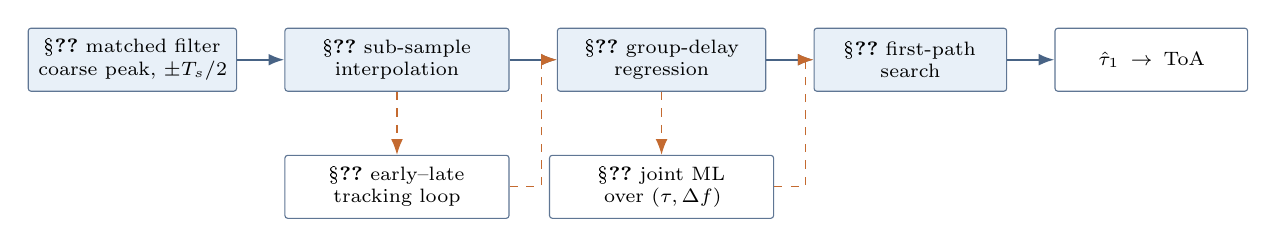
\begin{tikzpicture}[node distance=5mm and 6mm]
\node[blk,text width=24mm] (mf) {\S\ref{sec:mf} matched filter\\ coarse peak, $\pm T_s/2$};
\node[blk,right=of mf,text width=26mm] (interp) {\S\ref{sec:interp} sub-sample\\ interpolation};
\node[blk,right=of interp,text width=24mm] (fine) {\S\ref{sec:gd} group-delay\\ regression};
\node[blk,right=of fine,text width=22mm] (fp) {\S\ref{sec:firstpath} first-path\\ search};
\node[pblk,below=8mm of interp,text width=26mm] (el) {\S\ref{sec:el} early--late\\ tracking loop};
\node[pblk,below=8mm of fine,text width=26mm] (ml) {\S\ref{sec:ml} joint ML\\ over $(\tau,\Delta f)$};
\node[pblk,right=of fp,text width=22mm] (out) {$\hat\tau_1 \to \ToA$};
\draw[ar] (mf)--(interp); \draw[ar] (interp)--(fine); \draw[ar] (fine)--(fp); \draw[ar] (fp)--(out);
\draw[dar] (interp)--(el); \draw[dar] (el.east)-- ++(4mm,0) |- (fine.west);
\draw[dar] (fine)--(ml); \draw[dar] (ml.east) -- ++(4mm,0) |- (fp.west);
\end{tikzpicture}
\caption{Estimator composition. Solid path: the common acquire--refine--correct chain. Dashed:
optional refinements that replace or augment a stage.}
\label{fig:estchain}
\end{figure}

% ------------------------------------------------------------
\subsection{Matched filter and correlation peak}
\label{sec:mf}

Form the discrete cross-correlation of the received samples with the locally regenerated
reference $s[n]$:
\begin{equation}
R[m] \;=\; \sum_{n} z[n]\, s^{*}[n-m],
\qquad
\hat m \;=\; \arg\max_m \; \bigl|R[m]\bigr|^2 ,
\qquad
\hat\tau_{coarse} = \hat m\,T_s .
\label{eq:corr}
\end{equation}
Using $|R|^2$ rather than $\Re\{R\}$ makes the detector invariant to the unknown carrier phase
$\theta_0$. This is the non-coherent matched filter, and it is the maximum-likelihood detector for
a single path in white Gaussian noise with unknown phase.

\paragraph{Residual frequency offset.} A residual $\Delta f$ rotates the integrand and attenuates
the coherent peak by the factor $|\mathrm{sinc}(\Delta f\,T_{obs})|$. When
$\Delta f\, T_{obs}$ is not small, split the correlation into $K$ blocks and recombine
non-coherently:
\begin{equation}
\bigl|R_{nc}[m]\bigr|^2 \;=\; \sum_{k=1}^{K} \left| \sum_{n \in \mathcal{B}_k} z[n]\,s^{*}[n-m] \right|^2 .
\label{eq:noncoh}
\end{equation}
Each block must be short enough that $\Delta f\,T_{block} \ll 1$. Non-coherent combining costs
roughly $10\log_{10}K/2$\,dB of squaring loss at low SNR but tolerates an offset $K$ times larger.

\paragraph{Ambiguity.} The width of the main lobe of $|R[m]|$ is approximately $1/B \approx 500$\,ns
for a 2\,MHz packet. Sidelobe structure depends strongly on the reference: an access address is
DRBG-random and has a thumbtack autocorrelation with sidelobes near $1/\sqrt{32}$ of the peak,
whereas an alternating sounding sequence is periodic and has sidelobes approaching the peak at
multiples of the pattern period. Acquire on the access address; refine on the sequence.

% ------------------------------------------------------------
\subsection{Sub-sample interpolation}
\label{sec:interp}

Sampling at $F_{s,cal}=4$\,Msample/s gives $T_s = 250$\,ns. The reporting quantum is $0.5$\,ns, so
the interpolator must resolve to roughly $T_s/500$. This is entirely feasible because the
correlation peak is a smooth, known-shape function; the interpolation is a parameter fit, not a
resampling.

\paragraph{Parabolic (quadratic) interpolation.} With $y_i = |R[\hat m + i]|^2$ for $i\in\{-1,0,1\}$,
\begin{equation}
\hat\delta \;=\; \frac{1}{2}\,\frac{y_{-1} - y_{+1}}{y_{-1} - 2y_{0} + y_{+1}},
\qquad
\hat\tau \;=\; (\hat m + \hat\delta)\,T_s .
\label{eq:parab}
\end{equation}
Cheap and well conditioned, but biased: the true peak of $|R|^2$ for a band-limited signal is not a
parabola, so $\hat\delta$ exhibits an S-curve bias of up to a few percent of $T_s$ that is periodic
in the true fractional delay. The bias is deterministic and can be removed by a lookup table
calibrated on noise-free simulated waveforms.

\paragraph{Gaussian interpolation.} Replacing $y_i$ by $\ln y_i$ in Eq.~\eqref{eq:parab} fits a
Gaussian rather than a parabola. For a Gaussian-shaped pulse -- which the GFSK frequency pulse
approximately is -- this reduces the S-curve bias substantially at no extra cost.

\paragraph{Band-limited (sinc) interpolation.} The unbiased method. Zero-pad the correlation in the
frequency domain by a factor $L$, or equivalently apply a polyphase interpolation filter, and
re-locate the peak on the dense grid. Cost scales with $L$; a two-stage approach (parabolic to
within $T_s/10$, then a short sinc kernel over $\pm 2$ samples) achieves near-unbiased performance
at modest cost.

\paragraph{Oversampling requirement.} Sub-sample interpolation only recovers what Nyquist preserved.
If the anti-alias filter has removed spectral content, no interpolator restores the timing
information it carried. A practical receiver oversamples the 2\,MHz signal by at least $2\times$ and
preferably $4\times$ before correlating.

\begin{callout}
\textbf{Interpolate the magnitude, not the samples.} A common implementation error is to interpolate
the complex samples $z[n]$ and re-correlate. This is both more expensive and worse conditioned than
interpolating $|R[m]|^2$, which is real, positive, and smooth by construction.
\end{callout}

% ------------------------------------------------------------
\subsection{Early--late gate and delay-locked tracking}
\label{sec:el}

Rather than searching a grid, a tracking loop drives a timing error signal to zero. With an
early--late spacing $\Delta$,
\begin{equation}
e \;=\; \bigl|R(\hat\tau - \Delta)\bigr| - \bigl|R(\hat\tau + \Delta)\bigr|,
\qquad
\hat\tau \leftarrow \hat\tau - \mu\, e .
\label{eq:el}
\end{equation}
A normalised variant divides $e$ by $|R(\hat\tau)|$ to make the loop gain independent of received
amplitude, which matters because AGC settling changes the amplitude within a packet.

The sign convention is such that a positive $e$ means the estimate is late, hence the negative
update. The discriminator is linear over $|\tau - \hat\tau| < \Delta$, and its slope, and hence the
loop gain, depends on the correlation shape. Narrowing $\Delta$ steepens the discriminator and
reduces \emph{both} the thermal jitter and the multipath error envelope -- multipath mitigation is
the whole motivation for the narrow correlator. Its costs are a smaller pull-in range and a
requirement for wider pre-correlation bandwidth, since a narrow gate needs a sharp correlation peak.
A wide spacing pulls in over a larger range but is noisier and far more susceptible to multipath
capture.

Within a single Mode-1 step there is not enough signal to run a meaningful loop. The value of
Eq.~\eqref{eq:el} in Channel Sounding is \emph{across} steps: the per-step estimate from
Section~\ref{sec:interp} can seed a loop that tracks the range over a subevent or a procedure,
providing outlier rejection and smoothing at the cost of tracking lag on a moving target.

% ------------------------------------------------------------
\subsection{Maximum-likelihood estimation}
\label{sec:ml}

For the single-path model with unknown complex amplitude and unknown residual frequency, the
log-likelihood reduces to a two-dimensional search:
\begin{equation}
(\hat\tau, \widehat{\Delta f}) \;=\;
\arg\max_{\tau,\Delta f}\;
\left| \sum_n z[n]\, s^{*}\!\left(\tfrac{n}{F_{s,cal}} - \tau\right) e^{-j2\pi \Delta f\, n / F_{s,cal}} \right|^2 .
\label{eq:ml}
\end{equation}
Practically this is evaluated as a coarse FFT over $\Delta f$ at each candidate $\tau$ near the
correlation peak, followed by a local Newton or golden-section refinement in $\tau$. The frequency
search is inexpensive because Mode-0 has already reduced $\Delta f$ to a narrow interval.

For the multipath model, the ML problem becomes a joint estimation of $\{a_\ell,\tau_\ell\}$. Direct
optimisation is intractable, but the space-alternating generalised expectation-maximisation (SAGE)
algorithm decomposes it into a sequence of single-path problems: estimate the strongest component,
subtract it, re-estimate the next, and iterate. Applied to Mode-1 this is the principled version of
the ad-hoc leading-edge searches in Section~\ref{sec:firstpath}, and it is the method of choice
when computation permits.

% ------------------------------------------------------------
\subsection{Frequency-domain group-delay regression}
\label{sec:gd}

Transform both the received segment and the reference, and form the channel estimate over the
in-band bins $k$:
\begin{equation}
H[k] \;=\; \frac{Z[k]}{S[k]},
\qquad
\psi_k = \mathrm{unwrap}\bigl(\arg H[k]\bigr).
\label{eq:Hk}
\end{equation}
A pure delay $\tau$ produces $\psi_k = -2\pi f_k \tau + \psi_0$, so a weighted least-squares fit
gives
\begin{equation}
\hat\tau \;=\; -\frac{1}{2\pi}\,
\frac{\sum_k w_k (f_k - \bar f_w)(\psi_k - \bar\psi_w)}
     {\sum_k w_k (f_k - \bar f_w)^2},
\qquad
w_k \propto |S[k]|^2 .
\label{eq:gdreg}
\end{equation}

This is the exact frequency-domain dual of the unwrapped-phase time regression used in Mode-0: there
the observable is phase versus \emph{time} and the slope is a frequency; here it is phase versus
\emph{frequency} and the slope is a delay. The same practical cautions apply. Phase unwrapping fails
at low SNR and must be seeded by the coarse correlation estimate. Bins where $|S[k]|$ is small must
be down-weighted or excluded, which is why $w_k \propto |S[k]|^2$ rather than uniform weighting.
The residual after the fit is a valuable diagnostic: a systematically curved residual indicates
unresolved multipath rather than noise.

\begin{callout}
\textbf{Why this matters architecturally.} Equation~\eqref{eq:gdreg} over one packet's 2\,MHz is
exactly the operation Mode-2 phase-based ranging performs over the whole hopped band. Mode-1 and
Mode-2 are the same estimator applied over apertures that differ by a factor of forty in bandwidth.
That factor is precisely the ratio of their resolutions -- and the reason one is unambiguous and
the other is not.
\end{callout}

% ------------------------------------------------------------
\subsection{First-path detection under multipath}
\label{sec:firstpath}

In any indoor channel the strongest component is frequently not the earliest. Because the peak
estimator returns the strongest, the resulting delay error is \emph{one-sided and positive}: the
estimated range is biased long, never short. This is the dominant error in real deployments and is
the reason a raw correlation peak is not adequate for accurate ranging.

\paragraph{Back-search thresholding.} Locate the peak $|R|_{max}$, then search backwards in time for
the earliest sample exceeding $\alpha\,|R|_{max}$ within a window $W$:
\begin{equation}
\hat m_1 \;=\; \min\Bigl\{\, m \in [\hat m - W,\ \hat m] \;:\; |R[m]| \ge \alpha\,|R|_{max} \Bigr\}.
\label{eq:jbsf}
\end{equation}
The threshold $\alpha$ trades bias against false early detection on noise. Typical values lie
between $0.4$ and $0.7$; the correct value depends on the sidelobe level of the reference waveform
and must be characterised, not guessed.

\paragraph{CFAR leading edge.} Replace the fixed $\alpha$ by a threshold derived from a local noise
estimate taken from a pre-arrival guard region, so that the probability of an early false alarm is
held constant as SNR varies. This is markedly more robust than fixed thresholding across the
operating range.

\paragraph{Successive cancellation (CLEAN).} Iteratively estimate the strongest component, subtract
its contribution $\hat a\, s(t-\hat\tau)$ from the received signal, and repeat. The earliest
component surviving a significance test is taken as $\tau_1$. This is SAGE without the
re-estimation step and is a good cost compromise.

\paragraph{Super-resolution (informative).} Treating $H[k]$ from Eq.~\eqref{eq:Hk} as a spatial
snapshot, subspace methods -- MUSIC, root-MUSIC, ESPRIT -- or sparse recovery over a delay
dictionary (orthogonal matching pursuit, LASSO) can separate components closer than $1/B$. Over a
single Mode-1 packet the aperture is only 2\,MHz and the practical benefit is limited. The methods
become powerful only when $H[k]$ is stitched across many CS channels, which requires exactly the
frequency and phase coherency that Mode-0 and the PCT procedure provide. In other words,
super-resolution first-path detection is a cross-mode operation, not a Mode-1 operation.

\begin{callout}
\textbf{Bias is one-sided; exploit it.} Because multipath can only delay the estimate, a robust
combiner across steps should not use the mean. The minimum, or a low quantile, of the per-step
delay estimates is closer to the truth than the average whenever multipath bias exceeds thermal
noise. See Section~\ref{sec:agg}.
\end{callout}

% ------------------------------------------------------------
\subsection{Non-coherent and GFSK-specific methods}
\label{sec:gfsk}

\paragraph{Frequency-discriminator correlation.} A low-complexity receiver computes the instantaneous
frequency $y[n] = \arg\bigl(z[n]z^{*}[n-1]\bigr)$ and correlates it against the expected frequency
trajectory of the known bit pattern. This removes the unknown carrier phase and much of the residual
$\Delta f$ (as a constant offset in $y[n]$, easily removed by mean subtraction), at a cost of
roughly 2--3\,dB relative to the complex matched filter, worsening at low SNR because the
discriminator is nonlinear in noise.

\paragraph{Symbol timing recovery.} Classical timing-error detectors provide an independent estimate
of the symbol epoch: the Gardner detector, $e_k = \Re\{(z_k - z_{k-1})\,z^{*}_{k-1/2}\}$, is
attractive here because it is insensitive to carrier phase and works at two samples per symbol; the
Mueller--M\"uller detector needs only one sample per symbol but requires carrier phase lock. Timing
recovery alone yields the symbol epoch modulo $T_b$; the access-address correlation resolves which
symbol.

\paragraph{Zero-crossing timing.} An alternating sounding sequence at $h=0.5$ produces a waveform
whose instantaneous frequency alternates between $\pm R_b/4$, giving dense, regular zero crossings
in the discriminator output. Averaging the crossing positions over the sequence is a very cheap
timing estimator whose variance falls as $1/N$. It is biased by any DC offset in the discriminator
and by asymmetry in the modulator, both of which are calibratable.

% ------------------------------------------------------------
\subsection{The Cram\'er--Rao bound}
\label{sec:crlb}

For a known signal in additive white Gaussian noise, the delay estimation variance is bounded by
\begin{equation}
\sigma_\tau \;\ge\; \frac{1}{2\pi\,\beta_{rms}\,\sqrt{2\,\mathcal{E}/N_0}},
\qquad
\beta_{rms}^2 \;=\; \frac{\displaystyle\int f^2 |S(f)|^2\,df}{\displaystyle\int |S(f)|^2\,df},
\label{eq:crlb}
\end{equation}
where $\mathcal{E}/N_0$ is the \emph{accumulated} signal energy to noise density over the whole
observation. Writing $\mathcal{E}/N_0 = N\,\gamma$ with $N$ modulated symbols at per-symbol SNR
$\gamma$,
\begin{equation}
\sigma_\tau \;\ge\; \frac{1}{2\pi\,\beta_{rms}\sqrt{2N\gamma}} .
\label{eq:crlb2}
\end{equation}

Three levers appear, and only three: bandwidth, sequence length, and SNR. Bandwidth is fixed by the
PHY. Sequence length is the RTT type. SNR is the link. Everything an implementer can do beyond that
is to approach the bound rather than exceed it.

Propagating to the round-trip observable, the two directions are independent, so
\begin{equation}
\sigma_{\RTT} = \sqrt{\sigma_{\tau,I}^2 + \sigma_{\tau,R}^2} \;=\; \sqrt{2}\,\sigma_\tau
\quad\text{(symmetric links)},
\qquad
\sigma_d \;=\; \frac{c}{2}\,\sigma_{\RTT}.
\label{eq:sigmad}
\end{equation}
Averaging $M$ independent steps reduces $\sigma_d$ by $\sqrt{M}$ but does nothing to $D_{loop}$
error or multipath bias.

\begin{table}[h]
\caption{Cram\'er--Rao ranging standard deviation from Eqs.~\eqref{eq:crlb2}--\eqref{eq:sigmad}, using
$\beta_{rms}=0.50$\,MHz for the LE 2M PHY and $0.25$\,MHz for the LE 1M PHY. $\sigma_d$ is the
single-step value; the last column averages $M=32$ steps. These are bounds, not achieved
performance.}
\label{tab:crlb}
\centering\small
\begin{tabular}{@{}llrrrr@{}}
\toprule
PHY & Sequence & $\gamma$ & $\sigma_\tau$ (ns) & $\sigma_d$ (m) & $\sigma_d$, $M{=}32$ (cm) \\
\midrule
LE 2M & 96-bit & 30\,dB & $0.73$ & $0.154$ & $2.7$ \\
LE 2M & 96-bit & 20\,dB & $2.30$ & $0.487$ & $8.6$ \\
LE 2M & 96-bit & 10\,dB & $7.26$ & $1.540$ & $27.2$ \\
LE 2M & 32-bit & 20\,dB & $3.98$ & $0.844$ & $14.9$ \\
LE 1M & 96-bit & 20\,dB & $4.59$ & $0.974$ & $17.2$ \\
LE 1M & 32-bit & 20\,dB & $7.96$ & $1.687$ & $29.8$ \\
\bottomrule
\end{tabular}
\end{table}

\begin{callout}
\textbf{Reading Table~\ref{tab:crlb}.} Moving from a 32-bit to a 96-bit sequence buys
$\sqrt{3}\approx 1.7\times$; moving from the 1M to the 2M PHY buys $2\times$ through $\beta_{rms}$;
each 6\,dB of SNR buys $2\times$; each quadrupling of the step count buys $2\times$. Sub-decimetre
RTT-only ranging therefore requires good SNR \emph{and} a long sequence \emph{and} many steps -- and
still delivers only what an uncorrected 10\,ns loop delay would destroy fifteen times over.
\end{callout}

% ------------------------------------------------------------
\subsection{Comparison of estimators}

Table~\ref{tab:estcmp} summarises the family. No single row is a complete receiver: the practical
design is a chain of three or four of them, chosen so that each stage's weakness is covered by the
stage before it.

\begin{table}[htb]
\caption{Estimator comparison.}
\label{tab:estcmp}
\centering\small
\begin{tabular}{@{}L{34mm}L{30mm}L{30mm}L{26mm}@{}}
\toprule
Method & Strength & Weakness & Typical role \\
\midrule
Matched-filter peak (\S\ref{sec:mf}) & Robust, unambiguous with AA reference & Sample-grid resolution only & Acquisition \\
Parabolic interpolation (\S\ref{sec:interp}) & Negligible cost & Deterministic S-curve bias & Default refinement \\
Gaussian / sinc interpolation & Near-unbiased & Higher cost & Precision refinement \\
Early--late loop (\S\ref{sec:el}) & Smooths across steps & Tracking lag; multipath capture & Cross-step tracking \\
Joint ML (\S\ref{sec:ml}) & Attains the bound & Two-dimensional search & Reference implementation \\
Group-delay regression (\S\ref{sec:gd}) & Uses full bandwidth; diagnostic residual & Unwrapping fragile at low SNR & Refinement + QC \\
Back-search / CFAR (\S\ref{sec:firstpath}) & Removes one-sided multipath bias & Threshold must be characterised & Bias correction \\
SAGE / CLEAN & Principled multipath handling & Highest cost & High-accuracy mode \\
Super-resolution & Resolves close paths & Needs cross-channel aperture & Post-processing \\
Discriminator correlation (\S\ref{sec:gfsk}) & Very low cost & 2--3\,dB loss & Constrained receivers \\
\bottomrule
\end{tabular}
\end{table}

% ============================================================
\section{Reference estimation procedure for one Mode-1 step}
% ============================================================

The following is a complete implementation path, not a mandated algorithm.

\begin{enumerate}[label=\textbf{P\arabic*.},leftmargin=2.6em,itemsep=2pt]
  \item Compute the expected carrier for this step from the Mode-0 subevent reference and the
    channel's nominal centre; programme the LO and open the receive window with margins that bound
    the worst-case arrival uncertainty.
  \item Regenerate the step's access address, trailer, and sounding or random sequence from the CS
    DRBG state; synthesise the complex reference $s[n]$ at the working sample rate.
  \item Capture $z[n]$ across the window; record AGC state, gain changes and any clipping.
  \item Correlate per Eq.~\eqref{eq:corr}, using non-coherent block combining
    (Eq.~\eqref{eq:noncoh}) if the residual frequency uncertainty warrants it. Detect on the access
    address portion only.
  \item Validate detection: peak-to-sidelobe ratio above threshold, peak within the expected window,
    estimated SNR above the configured floor.
  \item Refine to sub-sample resolution (Eq.~\eqref{eq:parab} or its unbiased variants), then, if the
    RTT type provides a sequence, extend the correlation aperture over the full packet and re-refine.
  \item Optionally run the group-delay regression (Eq.~\eqref{eq:gdreg}) over the in-band bins; retain
    the fit residual as a quality metric.
  \item Run first-path correction (Eq.~\eqref{eq:jbsf} or CLEAN) and record both the peak-based and
    the first-path-based estimates, so the bias correction can be audited.
  \item Convert to an antenna-referenced arrival time by subtracting the calibrated receive group
    delay for this channel, PHY, RTT type and gain state.
  \item Apply the sample-clock scale correction: an estimator output expressed in samples must be
    converted using the calibrated physical $F_{s,cal}$, not the nominal rate.
  \item Quantise to the reporting resolution only at the interface boundary. Retain full precision
    internally.
  \item Emit the record
    $\{k,\ \text{channel},\ \ToA,\ \ToD,\ \text{peak SNR},\ \text{PSR},\ \text{fit residual},\
    \text{first-path offset},\ \NADM,\ \text{flags}\}$.
\end{enumerate}

% ============================================================
%  Sections 11-18, appendices, references
% ============================================================

% ============================================================
\section{Aggregation of Mode-1 steps}
\label{sec:agg}
% ============================================================

\subsection{Per-step validity gating}

Let $y_k$ be the corrected round-trip time of step $k$ from Eq.~\eqref{eq:rttfinal}, and $g_k \in
\{0,1\}$ a validity gate. A step should be gated out, or heavily down-weighted, when any of the
following holds: the correlation peak-to-sidelobe ratio is below threshold; the estimated SNR is
below the configured floor; the peak lies outside the expected arrival window; the group-delay fit
residual is inconsistent with a single dominant path; the AGC changed state during the reference
sequence; clipping occurred; the reflector reported its measurement as unavailable; or the
$\NADM$ indicates a probable attack.

\subsection{Weighted combination}

With $\sigma_k$ an uncertainty estimate for step $k$ and a variance floor $\sigma_{floor}$
representing the irreducible calibration and multipath contribution,
\begin{equation}
w_k \;=\; g_k \min\!\left( w_{max},\ \frac{1}{\sigma_k^2 + \sigma_{floor}^2} \right),
\qquad
\widehat{\RTT} \;=\; \frac{\sum_{k=1}^{M} w_k\, y_k}{\sum_{k=1}^{M} w_k}.
\label{eq:agg}
\end{equation}
The floor and the cap $w_{max}$ prevent a single optimistic step from dominating, which is the
standard failure mode of purely inverse-variance weighting when $\sigma_k$ is itself estimated from
the data.

\subsection{Robust and bias-aware combination}

Equation~\eqref{eq:agg} is the right estimator for zero-mean errors. Multipath error is not
zero-mean: it is one-sided and positive (Section~\ref{sec:firstpath}). Where multipath bias
dominates thermal noise, a lower-quantile combiner is better conditioned:
\begin{equation}
\widehat{\RTT}_{q} \;=\; Q_q\bigl(\{y_k : g_k = 1\}\bigr), \qquad q \approx 0.1\ \text{to}\ 0.3 ,
\label{eq:quantile}
\end{equation}
possibly with a small positive offset calibrated to remove the resulting downward bias of the
quantile itself. The correct choice depends on the ratio of thermal to multipath error, which
varies with SNR and environment, so a practical implementation computes both and selects using the
observed scatter of $\{y_k\}$: scatter close to the predicted thermal value indicates a clean
channel where the weighted mean is right; scatter much larger than predicted, with a long right
tail, indicates multipath, where the quantile is right.

Additional records worth retaining alongside the estimate: the accepted step count, the channel
span covered, the residual scatter, the maximum within-subevent deviation, and the estimate age.

% ============================================================
\section{Relationship to phase-based ranging}
\label{sec:fusion}
% ============================================================

Mode-1 and Mode-2 measure the same physical delay through different observables with complementary
failure modes.

\begin{table}[h]
\caption{Complementary character of the two ranging observables.}
\label{tab:fusion}
\centering\small
\begin{tabular}{@{}L{34mm}L{45mm}L{45mm}@{}}
\toprule
Property & Mode-1 (RTT) & Mode-2/3 (phase slope) \\
\midrule
Observable & Packet arrival time & Channel phase $2\theta_{CH}(f)$ vs.\ $f$ \\
Aperture & One packet, $\approx 2$\,MHz & Hopped band, up to $\approx 80$\,MHz \\
Resolution & $\approx 1/B \approx 500$\,ns & $\approx 1/B_{hop} \approx 12$\,ns \\
Ambiguity & None over the operating range & Periodic; unambiguous range set by channel spacing \\
Dominant error & Thermal jitter; loop delay bias & LO phase, multipath, frequency drift \\
Needs from Mode-0 & Clock scale for $B_R$; carrier placement & Residual frequency for phase drift \\
\bottomrule
\end{tabular}
\end{table}

The natural fusion is therefore hierarchical: the Mode-1 estimate selects the correct ambiguity
interval of the phase-based estimate, and the phase-based estimate supplies the precision within it.
For this to work, the Mode-1 uncertainty must be smaller than half the phase ambiguity interval.
With a 1\,MHz channel spacing the phase observable repeats every $c/(2\cdot 1\,\text{MHz}) = 150$\,m
of distance, which Mode-1 clears easily. Where the measured channel subset leaves a sparser effective
spacing, the ambiguity interval shrinks, the requirement tightens, and Table~\ref{tab:crlb} becomes
the governing constraint on how much averaging the RTT stage needs.

% ============================================================
\section{Timing integrity: markers and the attack detector}
% ============================================================

\subsection{Threat model}

The relevant attack against a round-trip time measurement is distance reduction. An adversary
cannot make a legitimate signal arrive earlier, but it can make a receiver \emph{believe} the signal
arrived earlier, by transmitting a guessed continuation of the packet before the genuine one is
complete. This is the early-detect/late-commit (EDLC) family: detect the earliest symbols, guess the
rest, and commit a forged waveform in advance.

The countermeasures are structural. The access address is DRBG-derived per step, so the attacker
cannot precompute it. The random sequence types make the entire payload unpredictable. The sounding
sequence types are predictable in their bulk pattern but carry 4-bit markers at positions the
attacker does not know, so a forged continuation will disagree with the genuine waveform exactly
where it is checked.

\subsection{The Normalized Attack Detector Metric}

$\NADM$ quantifies how far a received GFSK waveform departs from the waveform the receiver expected,
after the timing and frequency estimates have been applied. Conceptually it is a normalised residual:
\begin{equation}
\NADM \;\propto\; \frac{\bigl\| z - \hat a\, s(\cdot - \hat\tau)\,e^{\,j\hat\phi} \bigr\|^2}
                        {\bigl\| z \bigr\|^2},
\label{eq:nadm}
\end{equation}
mapped through an implementation-specific characterisation onto a small ordinal scale reported per
step. A clean signal produces a residual consistent with the estimated noise level; a spliced or
forged waveform produces a structured residual concentrated at the marker positions and at the
splice point.

\begin{table}[h]
\caption{Reported $\NADM$ scale. The mapping from Eq.~\eqref{eq:nadm} onto these levels is an
implementation characterisation, not a specified formula.}
\label{tab:nadm}
\centering\small
\begin{tabular}{@{}cl@{\hspace{12mm}}cl@{}}
\toprule
Value & Interpretation & Value & Interpretation \\
\midrule
0x00 & Attack extremely unlikely & 0x04 & Attack likely \\
0x01 & Attack very unlikely      & 0x05 & Attack very likely \\
0x02 & Attack unlikely           & 0x06 & Attack extremely likely \\
0x03 & Attack possible           & 0xFF & Unknown \\
\bottomrule
\end{tabular}
\end{table}

\subsection{Estimator interaction}

There is a real tension between accuracy and integrity, and it should be stated plainly. Every
first-path technique in Section~\ref{sec:firstpath} deliberately pulls the estimate \emph{earlier}
than the correlation peak in order to remove multipath bias. That is precisely the direction an
attacker wants to push it. A back-search threshold set aggressively for multipath performance widens
the window in which a forged early arrival is accepted.

The resolution is to keep the two decisions separate and to record both: perform detection and
$\NADM$ evaluation against the full expected waveform including markers, and perform first-path
correction only within a window whose extent is justified by the channel model and is reported
alongside the result. A first-path correction larger than the plausible multipath spread should
raise the same suspicion as a poor $\NADM$.

% ============================================================
\section{Worked numerical example at 2\,440\,MHz}
\label{sec:example}
% ============================================================

Assume the LE 2M PHY, RTT type 0x02 (96-bit sounding sequence), $\Tip = 145\us$, $\Trd = 5\us$,
receiver sample rate $F_{s,cal} = 4$\,Msample/s, per-symbol SNR $\gamma = 20$\,dB, $M = 32$ valid
Mode-1 steps, and a true separation of $d = 10.000$\,m.

\subsection{Nominal timing}

From Table~\ref{tab:tsy}, $\Tsy = 74\us$. From Eq.~\eqref{eq:stepdur},
\begin{equation}
T_{step,1} = 2(74) + 2(5) + 145 = 303\us .
\end{equation}
The reflector's turnaround interval, referenced to the access-address start of each packet, is
\begin{equation}
B_R \approx \Tsy + \Trd + \Tip = 224\us .
\end{equation}

\subsection{The quantity being measured}

\begin{align}
\ToF &= \frac{10.000}{299\,792\,458} = 33.356410\ \text{ns}, \\
\RTT &= 2\,\ToF = 66.712819\ \text{ns} .
\end{align}
This is $0.2669$ of one sample period at $F_{s,cal}$, and $0.1334$ of one symbol period at 2\,Mb/s.
The entire ranging observable is therefore a small fraction of a single sample interval: sub-sample
interpolation is not an optimisation in Mode-1, it is the measurement.

\subsection{Reporting quantum}

At a reporting resolution of $0.5$\,ns,
\begin{equation}
\frac{\RTT}{0.5\ \text{ns}} = 133.4256\ \text{LSB},
\qquad
1\ \text{LSB} \;\leftrightarrow\; \frac{c \times 0.5\ \text{ns}}{2} = 7.495\ \text{cm},
\end{equation}
and uniform rounding of one field contributes a standard deviation of
$0.5/\sqrt{12} = 0.1443$\,ns. Because Eq.~\eqref{eq:rttfinal} differences \emph{two} separately
quantised contributions (Appendix~\ref{app:hci}), the two independent roundings combine to
$0.5\sqrt{2/12} = 0.2041$\,ns, or $3.06$\,cm of range.

\subsection{Thermal limit}

From Eq.~\eqref{eq:crlb2} with $\beta_{rms} = 0.50$\,MHz, $N = 96$, $\gamma = 100$:
\begin{align}
\sigma_\tau     &= \frac{1}{2\pi (0.5\times10^{6})\sqrt{2 \times 96 \times 100}} = 2.297\ \text{ns},\\
\sigma_{\RTT}   &= \sqrt{2}\,\sigma_\tau = 3.249\ \text{ns}, \\
\sigma_d        &= \tfrac{c}{2}\,\sigma_{\RTT} = 0.487\ \text{m} \quad\text{(single step)}, \\
\sigma_d^{(32)} &= 0.487/\sqrt{32} = 8.61\ \text{cm}.
\end{align}

\subsection{Clock-scale term}

With $B_R = 224\us$ and Eq.~\eqref{eq:rescale} not applied, a 12\,ppm oscillator pair gives
\begin{equation}
\delta t = 224\times10^{-6}\times 12\times10^{-6} = 2.688\ \text{ns}
\quad\Rightarrow\quad
\delta d = 40.3\ \text{cm}.
\end{equation}
After a Mode-0 correction good to $0.05$\,ppm, the same term becomes $11.2$\,ps, or $1.7$\,mm --
comfortably below the thermal floor. Note that this error is a \emph{bias} common to every step on
that link, so averaging does not reduce it; only the Mode-0 correction does.

\subsection{Loop delay}

If $D_{loop}$ were left uncalibrated at a plausible $10$\,ns, the range would be biased by
\begin{equation}
\delta d = \frac{c \times 10\ \text{ns}}{2} = 1.499\ \text{m},
\end{equation}
which exceeds every other term combined by more than an order of magnitude. Calibrated to a residual
of $0.5$\,ns, the contribution falls to $7.5$\,cm, comparable to the thermal floor.

\subsection{Assembled budget}

\begin{table}[h]
\caption{Assembled uncertainty for the worked example: LE 2M PHY, 96-bit sounding sequence,
$\gamma = 20$\,dB, $M = 32$ steps, $\Tip = 145\us$. The root-sum-square is an upper-bound
convenience only: the rows marked as biases are common to every step on the link and are neither
reduced by averaging nor correctly combined in quadrature; see Eq.~\eqref{eq:budget}.}
\label{tab:example}
\centering\small
\begin{tabular}{@{}L{54mm}rrl@{}}
\toprule
Contribution & Time & Range & Character \\
\midrule
Thermal noise, 32 steps        & $0.574$\,ns & $8.61$\,cm & random \\
Loop-delay calibration residual& $0.500$\,ns & $7.49$\,cm & bias, per channel \\
Reporting quantisation, two fields & $0.204$\,ns & $3.06$\,cm & random \\
Sample-rate / interpolation bias& $0.067$\,ns & $1.00$\,cm & bias \\
Clock scale after Mode-0 (0.05\,ppm) & $0.011$\,ns & $0.17$\,cm & bias \\
\midrule
Root-sum-square (excluding multipath) & $0.791$\,ns & $11.9$\,cm & \\
\midrule
First-path multipath bias, indoor & typ.\ $+2$\,ns & $+30$\,cm & one-sided, environment \\
\bottomrule
\end{tabular}
\end{table}

The table carries the report's central practical message. Under favourable conditions the
instrumental terms combine to roughly a decimetre, and the residual multipath bias -- which is not
reduced by averaging and is not symmetric -- is then the largest single error. Effort spent on
first-path estimation and on loop-delay calibration buys more accuracy than effort spent on the
correlator.

\begin{table}[h]
\caption{Deterministic values for the 2\,440\,MHz example.}
\label{tab:exvalues}
\centering\small
\begin{tabular}{@{}L{60mm}rl@{}}
\toprule
Quantity & Value & Unit \\
\midrule
CS synchronization PHY & LE 2M & \\
RTT type & 0x02 (96-bit sounding sequence) & \\
$\Tsy$ & 74 & \us \\
$\Trd$ & 5 & \us \\
$\Tip$ & 145 & \us \\
Step duration $T_{step,1}$ & 303 & \us \\
Reflector turnaround $B_R$ & 224 & \us \\
True distance & 10.000 & m \\
One-way time of flight & 33.356410 & ns \\
Round-trip time & 66.712819 & ns \\
RTT in 0.5\,ns units & 133.4256 & LSB \\
RTT as a fraction of $T_s$ at 4\,Msps & 0.26685 & samples \\
Range per ns of RTT error & 0.14990 & m \\
Range per 0.5\,ns LSB & 0.07495 & m \\
CRLB $\sigma_\tau$ at 20\,dB & 2.297 & ns \\
CRLB $\sigma_d$, single step & 0.487 & m \\
CRLB $\sigma_d$, 32 steps & 0.0861 & m \\
Bias from 10\,ns uncalibrated $D_{loop}$ & 1.499 & m \\
Bias from 12\,ppm uncorrected clock scale & 0.403 & m \\
\bottomrule
\end{tabular}
\end{table}

% ============================================================
\section{Error sources and uncertainty}
% ============================================================

\begin{table}[h]
\caption{Representative Mode-1 timing error budget.}
\label{tab:errors}
\centering\small
\begin{tabular}{@{}L{30mm}L{34mm}L{34mm}L{30mm}@{}}
\toprule
Source & Effect & Mitigation & Diagnostic \\
\midrule
Thermal noise & Random delay jitter, $\propto 1/(\beta_{rms}\sqrt{N\gamma})$ & Longer sequence, 2M PHY, more steps & Scatter versus predicted CRLB \\
TX/RX group delay & Additive loop-delay bias, $c D_{loop}/2$ & Conducted calibration per channel, PHY, gain state & Cable loopback at known delay \\
Channel-dependent filter delay & Per-channel range offset & Calibration surface over channels & Range versus channel sweep \\
Temperature drift of $D_{loop}$ & Slow bias drift & Temperature-indexed table & Range versus temperature \\
AGC state change & Path change mid-packet & Freeze gain after preamble; per-gain calibration & Range versus input level \\
Residual carrier offset & Coherent-integration loss & Mode-0 correction; non-coherent blocking & Peak height versus injected offset \\
Clock-scale error & Bias $\propto \epsilon B_R$ & Mode-0 $\FFO^{*}_{RX}$ rescaling & Range versus $\Tip$ setting \\
Sign error in rescaling & Doubles the clock term & End-to-end signed injection test & Range versus injected ppm \\
Sample-rate error & Scale error in estimator output & Use calibrated $F_{s,cal}$ & Digital injection test \\
Interpolator S-curve & Periodic bias in fractional delay & Unbiased kernel or lookup correction & Range versus sub-sample delay sweep \\
Timestamp reference mismatch & Whole-symbol offsets & Common antenna-plane convention & Cross-vendor comparison \\
Multipath first path & One-sided positive bias & First-path search, CFAR, SAGE & Peak-to-first-path offset \\
Motion during step & Forward/return asymmetry & Bound by step duration; velocity model & Range rate consistency \\
Interference & Corrupted correlation & Gating on PSR and SNR & Rejected-step rate per channel \\
Non-reciprocal RF path & Uncancelled hardware delay & Calibrate with switch states used & Path-reversal test \\
EDLC attack & Reduced apparent distance & Random/sounding sequence, $\NADM$ & $\NADM$ distribution, marker check \\
\bottomrule
\end{tabular}
\end{table}

For approximately independent contributions the first-order budget is
\begin{equation}
\sigma_{\RTT}^2 \;\approx\; \sigma_{est}^2 + \sigma_{cal}^2 + \sigma_{q}^2 + \sigma_{scale}^2
   + \sigma_{clk}^2 ,
\label{eq:budget}
\end{equation}
with the multipath term handled separately because it is a bias rather than a variance. Correlated
terms must not be combined by blind root-sum-square: the loop-delay calibration residual, the
sample-rate error and the timestamp reference convention are all common to every step on a link, so
they survive averaging intact while $\sigma_{est}$ falls as $1/\sqrt{M}$.

% ============================================================
\section{Verification and conformance-oriented test plan}
% ============================================================

\subsection{Layered verification}

\begin{enumerate}[leftmargin=1.7em,itemsep=2pt]
  \item \textbf{Pure DSP vectors.} Synthesised \code{CS\_SYNC} waveforms at exactly known fractional
    delays, swept in fine steps across a full sample period, with AWGN, carrier offset, DC, I/Q
    imbalance and clipping. Verify that the estimated delay tracks the injected delay with bounded
    residual, and characterise the interpolator S-curve.
  \item \textbf{Multipath vectors.} Two- and three-path channels with controlled amplitude ratios
    and separations from $0.1/B$ to $3/B$. Verify the first-path estimator's bias and its failure
    threshold. Confirm the bias is one-sided.
  \item \textbf{Digital radio-loop vectors.} Inject after downconversion to verify sample-rate
    calibration, decimation offsets, and fixed-point arithmetic.
  \item \textbf{Conducted delay-line tests.} Two devices connected through calibrated cable lengths
    or a programmable delay line. This is the only test that measures $D_{loop}$ directly; sweep
    channel, temperature, input level and PHY.
  \item \textbf{Path-reversal test.} Repeat the conducted test with the roles of initiator and
    reflector exchanged. A difference in the result exposes non-reciprocal hardware delay.
  \item \textbf{Clock-scale tests.} Deliberately offset one device's reference by a known ppm value
    and verify that the measured range is invariant. Sweep the sign, and sweep $\Tip$ across its
    permitted set; a residual slope of range versus $\Tip$ is the signature of an uncorrected or
    wrongly signed clock term.
  \item \textbf{RTT-type coverage.} Repeat the accuracy characterisation for every supported RTT
    type; the loop delay is generally type-dependent because the estimator uses a different aperture.
  \item \textbf{Anechoic and multipath chamber tests.} Absolute accuracy at known geometric
    distances, then in a reverberant environment, to separate instrumental error from channel bias.
  \item \textbf{Attack injection.} Replay and EDLC-style forgeries; verify $\NADM$ responds and that
    the first-path window bounds the achievable distance reduction.
  \item \textbf{Aggregation tests.} Controlled outliers and gated steps; verify weighting, gating and
    the quantile combiner behave as specified, and that reported step counts match.
\end{enumerate}

\subsection{Minimum acceptance records}

Retain: RF configuration, CS channel list, PHY and RTT type, $\Tip$ and $T_{FCS}$ settings, the
applied $\FFO^{*}_{RX}$, calibrated $F_{s,cal}$, the $D_{loop}$ calibration table version, per-step
raw and corrected timing estimates, peak SNR and peak-to-sidelobe ratio, first-path correction
applied, $\NADM$, validity flags, aggregated result with accepted step count and scatter, and
pass/fail limits. Reproducible vectors should include the worked example of
Section~\ref{sec:example}, a fractional-delay sweep across one full sample period, a known
two-path case, and a known injected clock offset of each sign.

% ============================================================
\section{Normative behaviour versus implementation choice}
% ============================================================

Table~\ref{tab:normvsimpl} separates what the specification fixes from what the implementer decides.
The pattern is consistent with Mode-0: the specification fixes the air interface, the observables and
their meaning, while every estimator, quality metric and calibration mechanism is design freedom --
and is therefore where accuracy is won or lost.

\begin{table}[htb]
\caption{Boundary between specified behaviour and implementation design.}
\label{tab:normvsimpl}
\centering\small
\begin{tabular}{@{}L{62mm}L{62mm}@{}}
\toprule
Bluetooth-defined behaviour & Implementation-specific design \\
\midrule
Mode-1 exchange order; $\Tsy$, $\Trd$, $\Tip$, $T_{FCS}$ and their permitted sets & Receive window margins, sample rate, numeric format \\
\code{CS\_SYNC} construction: access address, trailer, sounding and random sequences & Reference waveform synthesis, matched-filter structure \\
RTT type definitions and capability negotiation & Which estimator is used for which type \\
Meaning of the reported timing observables and their resolution & Correlation, interpolation, ML, group-delay or hybrid estimator \\
Requirement that measurements be referenced consistently between devices & Choice of antenna-plane reference and its calibration \\
Use of the Mode-0 result for frequency and timing compensation & Rescaling arithmetic, precision, filtering of $\FFO^{*}_{RX}$ \\
$\NADM$ reporting and its scale & Metric computation, thresholds, characterisation \\
Per-step reporting and validity indication & Quality metrics, gating rules, aggregation and outlier policy \\
Relationship of RTT to the ranging procedure & Fusion with phase-based ranging, multipath model, tracking filter \\
\bottomrule
\end{tabular}
\end{table}

\begin{callout}
\textbf{Four conclusions that prevent common design errors.} (1) The reciprocal construction cancels
the reflector's turnaround but \emph{accumulates} all four hardware group delays into an additive
loop delay that must be calibrated. (2) The reflector's interval is measured on the reflector's
clock and must be rescaled by the Mode-0 fractional frequency offset before subtraction; the error
grows with $\Tip$. (3) Mode-1 accuracy is estimation-limited, not resolution-limited: the whole
observable at 10\,m is a quarter of one sample period, so sub-sample interpolation is the
measurement rather than a refinement. (4) Multipath error is one-sided and positive, so it is not
reduced by averaging and is not correctly handled by a mean.
\end{callout}

% ============================================================
\section{Conclusions}
% ============================================================

Mode-1 converts a reciprocal packet exchange into an unambiguous distance. The measurement is
structurally elegant: because each device times only its own events and the reflector reports what it
measured, the unknown turnaround time cancels exactly and only the propagation delay survives. That
elegance is bounded by two physical facts. Transmit and receive chain delays add rather than cancel,
so the accuracy of a Mode-1 range is ultimately the accuracy of a hardware calibration. And the two
intervals are measured with two different oscillators, so Mode-0 is not an optional preliminary but
a term in the equation.

The estimation problem itself is a known-signal delay estimation with a nuisance phase, a small
residual frequency offset, and an objective -- the first arriving path -- that is not the maximum of
the correlation. The estimator family that serves it is well understood: correlation for acquisition,
interpolation or group-delay regression for precision, maximum-likelihood or successive cancellation
for multipath, and cross-step aggregation that respects the one-sided character of the residual bias.
The Cram\'er--Rao bound ties the achievable precision to just three quantities -- root-mean-square
bandwidth, sequence length and accumulated signal-to-noise ratio -- and thereby tells an implementer
exactly which configuration choices matter.

Mode-1 is not a complete ranging solution on its own, and it is not intended to be. It supplies the
coarse, unambiguous, attack-resistant scale within which the phase-based modes deliver precision. A
scientifically complete implementation validates the timing chain and the phase chain separately, and
then validates their combination.

% ============================================================
\appendix
\section{Reported quantities at the host interface}
\label{app:hci}
% ============================================================

Per Mode-1 step, the controller reports a small set of fields to the host in the CS subevent result.
Their exact names, widths and encodings are defined in Core 6.3, Vol.\ 4, Part E; the summary below
is given to make the data flow concrete and should be checked against the specification revision in
force.

\begin{table}[h]
\caption{Per-step Mode-1 reported fields.}
\label{tab:hci}
\centering\small
\begin{tabular}{@{}L{40mm}L{34mm}L{50mm}@{}}
\toprule
Field & Encoding & Role \\
\midrule
Initiator timing difference & signed, $0.5$\,ns units & The initiator's $A_I$ contribution \\
Reflector timing difference & signed, $0.5$\,ns units & The reflector's $B_R$ contribution \\
Packet quality & implementation index & Gating input \\
Packet RSSI & dBm & SNR proxy, gating input \\
Packet $\NADM$ & ordinal, see Table~\ref{tab:nadm} & Integrity gating \\
Packet antenna & index & Multi-antenna calibration selection \\
Unavailable indicator & reserved value & Step must be gated out \\
\bottomrule
\end{tabular}
\end{table}

Two implementation notes follow from the encoding. First, the signed 16-bit field at $0.5$\,ns
resolution spans roughly $\pm 16.4\us$, which is far narrower than the largest permitted $\Tip$;
the reported quantity is therefore a differential referenced to the configured nominal step timing
rather than an absolute interval, and an implementation must confirm the exact reference before
forming Eq.~\eqref{eq:rttfinal}. Second, the reserved ``unavailable'' value must be tested for
explicitly; interpreting it as a numeric timing value produces a grossly wrong range rather than a
rejected step.

% ============================================================
\section{Numerical test vectors}
% ============================================================

\begin{enumerate}[label=\textbf{B\arabic*.},leftmargin=2.6em,itemsep=2pt]
  \item \textbf{Fractional-delay sweep.} At $F_{s,cal} = 4$\,Msample/s, synthesise the LE 2M
    \code{CS\_SYNC} waveform with a 96-bit sounding sequence at true delays
    $\tau = 0,\,5,\,10,\ldots,250$\,ns. Noise-free, the estimated delay must reproduce the injected
    delay to within the documented interpolator bias; the residual as a function of $\tau$ is the
    S-curve to be tabulated and removed.
  \item \textbf{Thermal consistency.} Repeat B1 at $\gamma = 10$, $20$ and $30$\,dB with 1\,000
    trials each. The sample standard deviation must lie within a documented margin of the
    Table~\ref{tab:crlb} values: $7.26$, $2.30$ and $0.73$\,ns.
  \item \textbf{Two-path bias.} Add a second component at $+150$\,ns with $0\,\mathrm{dB}$ and
    $+6\,\mathrm{dB}$ relative amplitude. The peak estimator must show a positive bias; the
    first-path estimator must reduce it. Record both.
  \item \textbf{Loop delay.} Insert a known $D_{loop}$ of $10.0$\,ns in the model and verify the
    reported range shifts by $1.499$\,m, and that the calibration removes it to the documented
    residual.
  \item \textbf{Clock scale.} With $\Tip = 145\us$ and $\Tsy = 74\us$, inject $\epsilon = +12$\,ppm.
    Uncorrected, the range must shift by $+0.403$\,m; with $\FFO^{*}_{RX}$ applied per
    Eq.~\eqref{eq:rescale}, the residual must fall below $2$\,mm. Repeat with $\epsilon = -12$\,ppm to
    catch a sign inversion.
  \item \textbf{End-to-end.} With $d = 10.000$\,m, all corrections applied and $M = 32$ steps at
    $\gamma = 20$\,dB, the aggregated estimate must have mean within the documented bias limit of
    $10.000$\,m and standard deviation near $8.6$\,cm.
\end{enumerate}

\clearpage
% ============================================================
\section*{References}
\addcontentsline{toc}{section}{References}
% ============================================================

\begin{enumerate}[label={[\arabic*]},leftmargin=2.2em,itemsep=3pt]
\item Bluetooth SIG, \emph{Bluetooth Core Specification, Version 6.3}, Vol.\ 1, Part A,
  ``Architecture, Change History, and Conventions,'' Sec.\ 9.1 ``Channel Sounding procedure'' and
  Sec.\ 9.2 ``Distance estimation based on phase and amplitude information,'' adopted 2026.\\
  {\small\url{https://www.bluetooth.com/wp-content/uploads/Files/Specification/HTML/Core_v6.3/out/en/architecture,-change-history,-and-conventions/architecture.html}}

\item Bluetooth SIG, \emph{Bluetooth Core Specification, Version 6.3}, Vol.\ 6, Part H,
  ``Channel Sounding,'' Sec.\ 4.3.2 ``CS step mode-1,'' Sec.\ 4.3 step timing, and Sec.\ 4.4
  \code{CS\_SYNC} packet construction, adopted 2026.\\
  {\small\url{https://www.bluetooth.com/wp-content/uploads/Files/Specification/HTML/Core_v6.3/out/en/low-energy-controller/channel-sounding.html}}

\item Bluetooth SIG, \emph{Bluetooth Core Specification, Version 6.3}, Vol.\ 6, Part A,
  ``Radio Physical Layer Specification,'' Sec.\ 3.5 ``Frequency measurement and generation in
  Channel Sounding,'' adopted 2026.\\
  {\small\url{https://www.bluetooth.com/wp-content/uploads/Files/Specification/HTML/Core_v6.3/out/en/low-energy-controller/radio-physical-layer-specification.html}}

\item Bluetooth SIG, ``Bluetooth Core 6.3 Technical Overview,'' Secs.\ 3.2--3.3, 2026.\\
  {\small\url{https://www.bluetooth.com/bluetooth-core-6-3-technical-overview/}}

\item Bluetooth SIG, ``Bluetooth Channel Sounding'' feature page and Core 6.0 feature overview.\\
  {\small\url{https://www.bluetooth.com/learn-about-bluetooth/feature-enhancements/channel-sounding/}}

\item Silicon Labs, ``Bluetooth LE Channel Sounding Fundamentals,'' Location Services
  documentation, and the CS stack API RTT-type enumeration.\\
  {\small\url{https://docs.silabs.com/rtl-lib/latest/rtl-lib-channel-sounding-fundamentals/}}

\item MathWorks, ``What Is Bluetooth Channel Sounding?,'' Bluetooth Toolbox documentation.\\
  {\small\url{https://www.mathworks.com/help/bluetooth/ug/what-is-bluetooth-channel-sounding.html}}

\item Texas Instruments, ``High Accuracy, Low Cost, Secure Ranging with Bluetooth,'' application
  report SWRA791.\\
  {\small\url{https://www.ti.com/lit/swra791}}

\item S. M. Kay, \emph{Fundamentals of Statistical Signal Processing: Estimation Theory}.
  Prentice Hall, 1993. (Cram\'er--Rao bound for time delay; matched filtering.)

\item H. L. Van Trees, \emph{Detection, Estimation, and Modulation Theory, Part I}. Wiley, 2001.
  (Ambiguity function; delay estimation accuracy and resolution.)

\item B. H. Fleury, M. Tschudin, R. Heddergott, D. Dahlhaus and K. I. Pedersen, ``Channel parameter
  estimation in mobile radio environments using the SAGE algorithm,'' \emph{IEEE J.\ Sel.\ Areas
  Commun.}, vol.\ 17, no.\ 3, pp.\ 434--450, 1999.

\item I. Guvenc and Z. Sahinoglu, ``Threshold-based TOA estimation for impulse radio UWB systems,''
  \emph{IEEE Int.\ Conf.\ on Ultra-Wideband}, 2005. (Leading-edge and back-search thresholding.)

\item F. M. Gardner, ``A BPSK/QPSK timing-error detector for sampled receivers,'' \emph{IEEE Trans.\
  Commun.}, vol.\ 34, no.\ 5, pp.\ 423--429, 1986.

\item P. A. Laurent, ``Exact and approximate construction of digital phase modulations by
  superposition of amplitude modulated pulses,'' \emph{IEEE Trans.\ Commun.}, vol.\ 34, no.\ 2,
  pp.\ 150--160, 1986. (Matched filtering of CPM/GFSK.)

\item M. Poturalski, M. Flury, P. Papadimitratos, J.-P. Hubaux and J.-Y. Le Boudec, ``Distance
  bounding with IEEE 802.15.4a: attacks and countermeasures,'' \emph{IEEE Trans.\ Wireless
  Commun.}, vol.\ 10, no.\ 4, pp.\ 1334--1344, 2011. (Early-detect/late-commit attack model.)
\end{enumerate}

\end{document}
